% To produce handouts, uncomment the following:
% \documentclass[handout]{beamer}
% \usepackage{pgfpages}
% \pgfpagesuselayout{2 on 1}[a4paper,border shrink=5mm]

\documentclass{beamer}

\usepackage[T1]{fontenc}
\usepackage{textcomp} 


\usepackage{futura}
\usetheme{Antibes}
\usecolortheme{beetle}
\xdefinecolor{myyellow}{rgb}{0.97, 0.90, 0.49}
\setbeamercolor{alerted text}{fg=myyellow}


\title{Categorization errors and differences in the quality of questions across countries}
\author{Daniel Oberski\\Willem Saris\\Jacques Hagenaars}
\institute
{
  \inst{}%
  Faculty of Social and Behavioural Sciences\\
  Tilburg University
  \and
  \inst{}%
  Survey Research Centre\\
  ESADE Barcelona, Universitat Ramon Llull\vspace{-1.2cm}
}
\date{}

\begin{document}

\begin{frame}
	\titlepage
	\begin{center}
	 
\includegraphics[width=4.3cm]{i/uvttransparent.png}\hspace{.3cm}
	 
\includegraphics[width=2.0cm]{i/esade.png}\hspace{.3cm}
	 
\includegraphics[width=2.8cm]{i/ess.pdf}	
  \end{center}	
\end{frame}

\section*{Outline}

%\begin{frame}
%\frametitle{Overview}
%	\tableofcontents
%\end{frame}

\section{Survey response model}

\begin{frame}
	\frametitle{The basic survey response model}
	\pause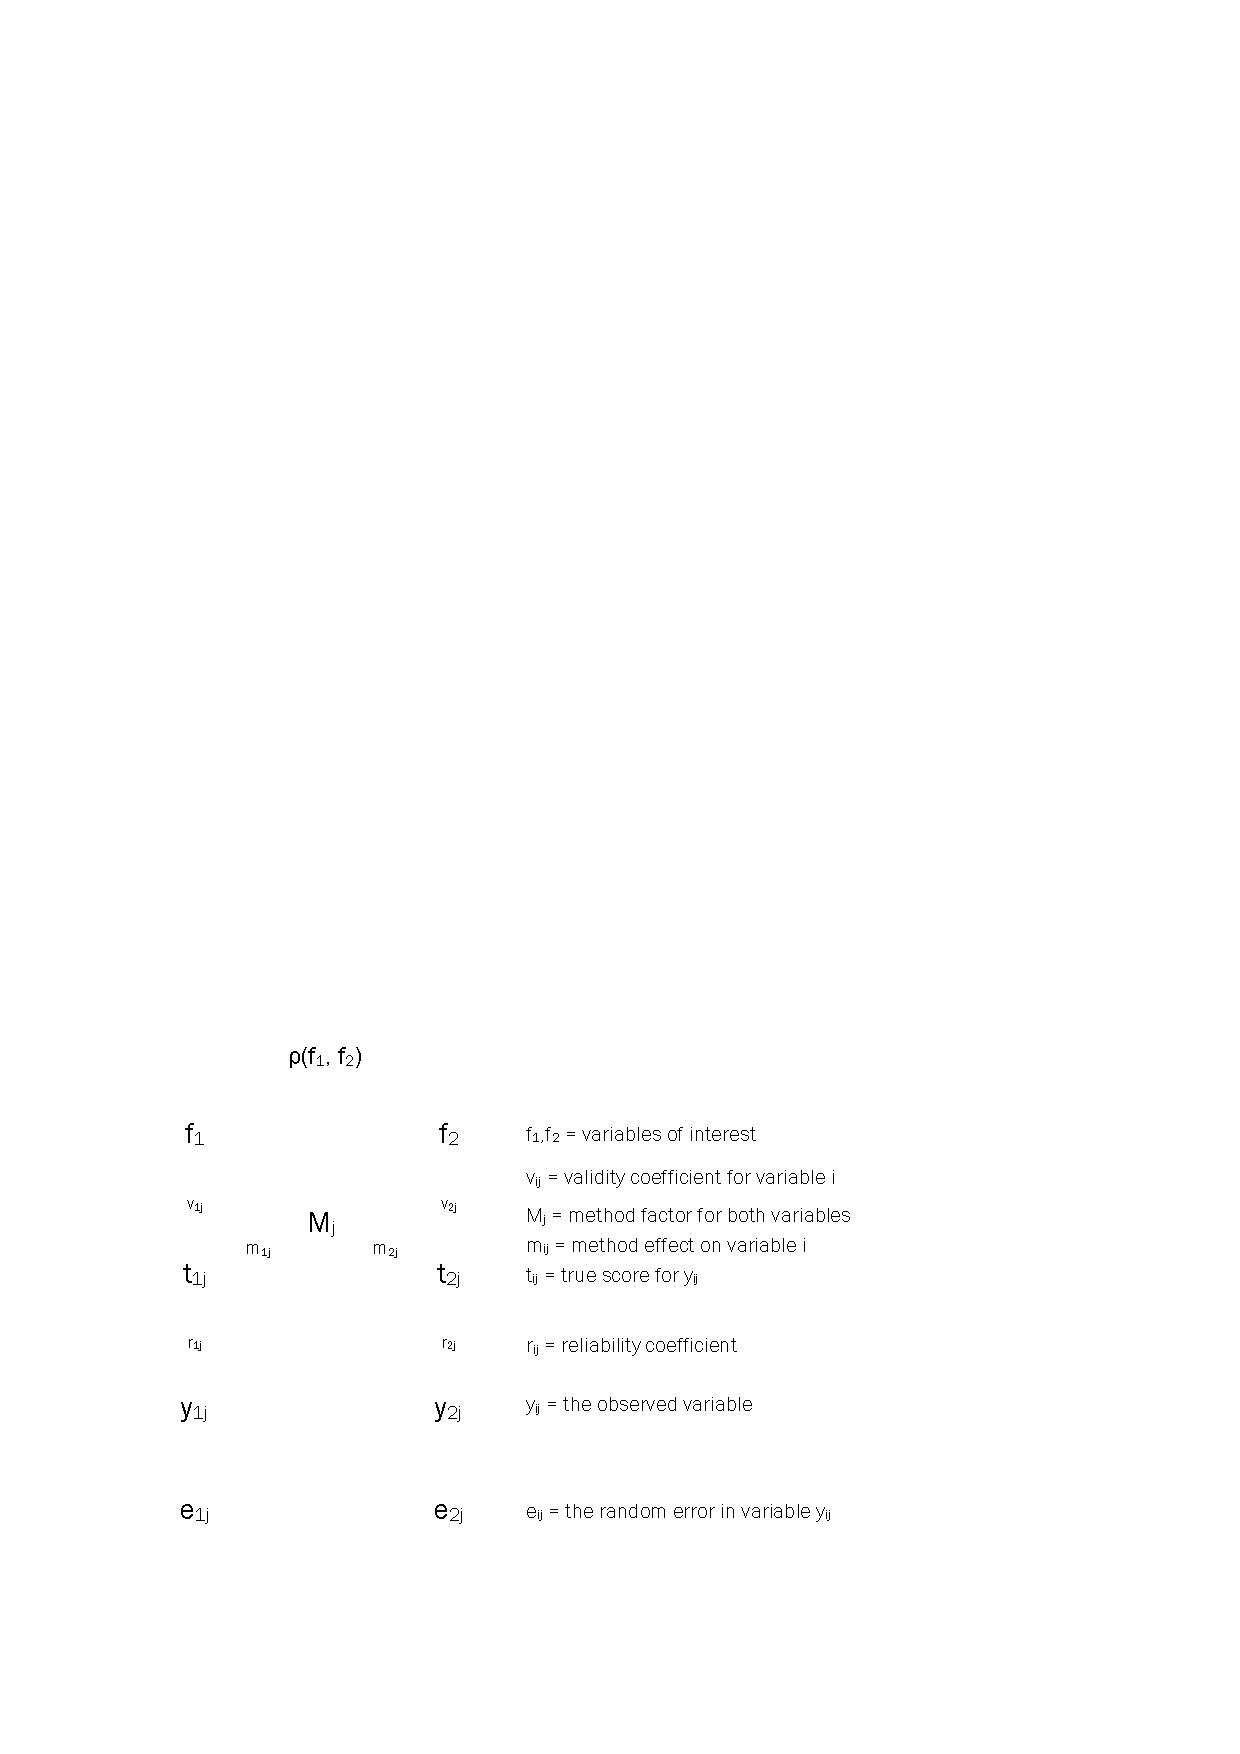
\includegraphics[height=7cm]{i/response-model.pdf}\\
\end{frame}

\subsection{Example}
\begin{frame}
	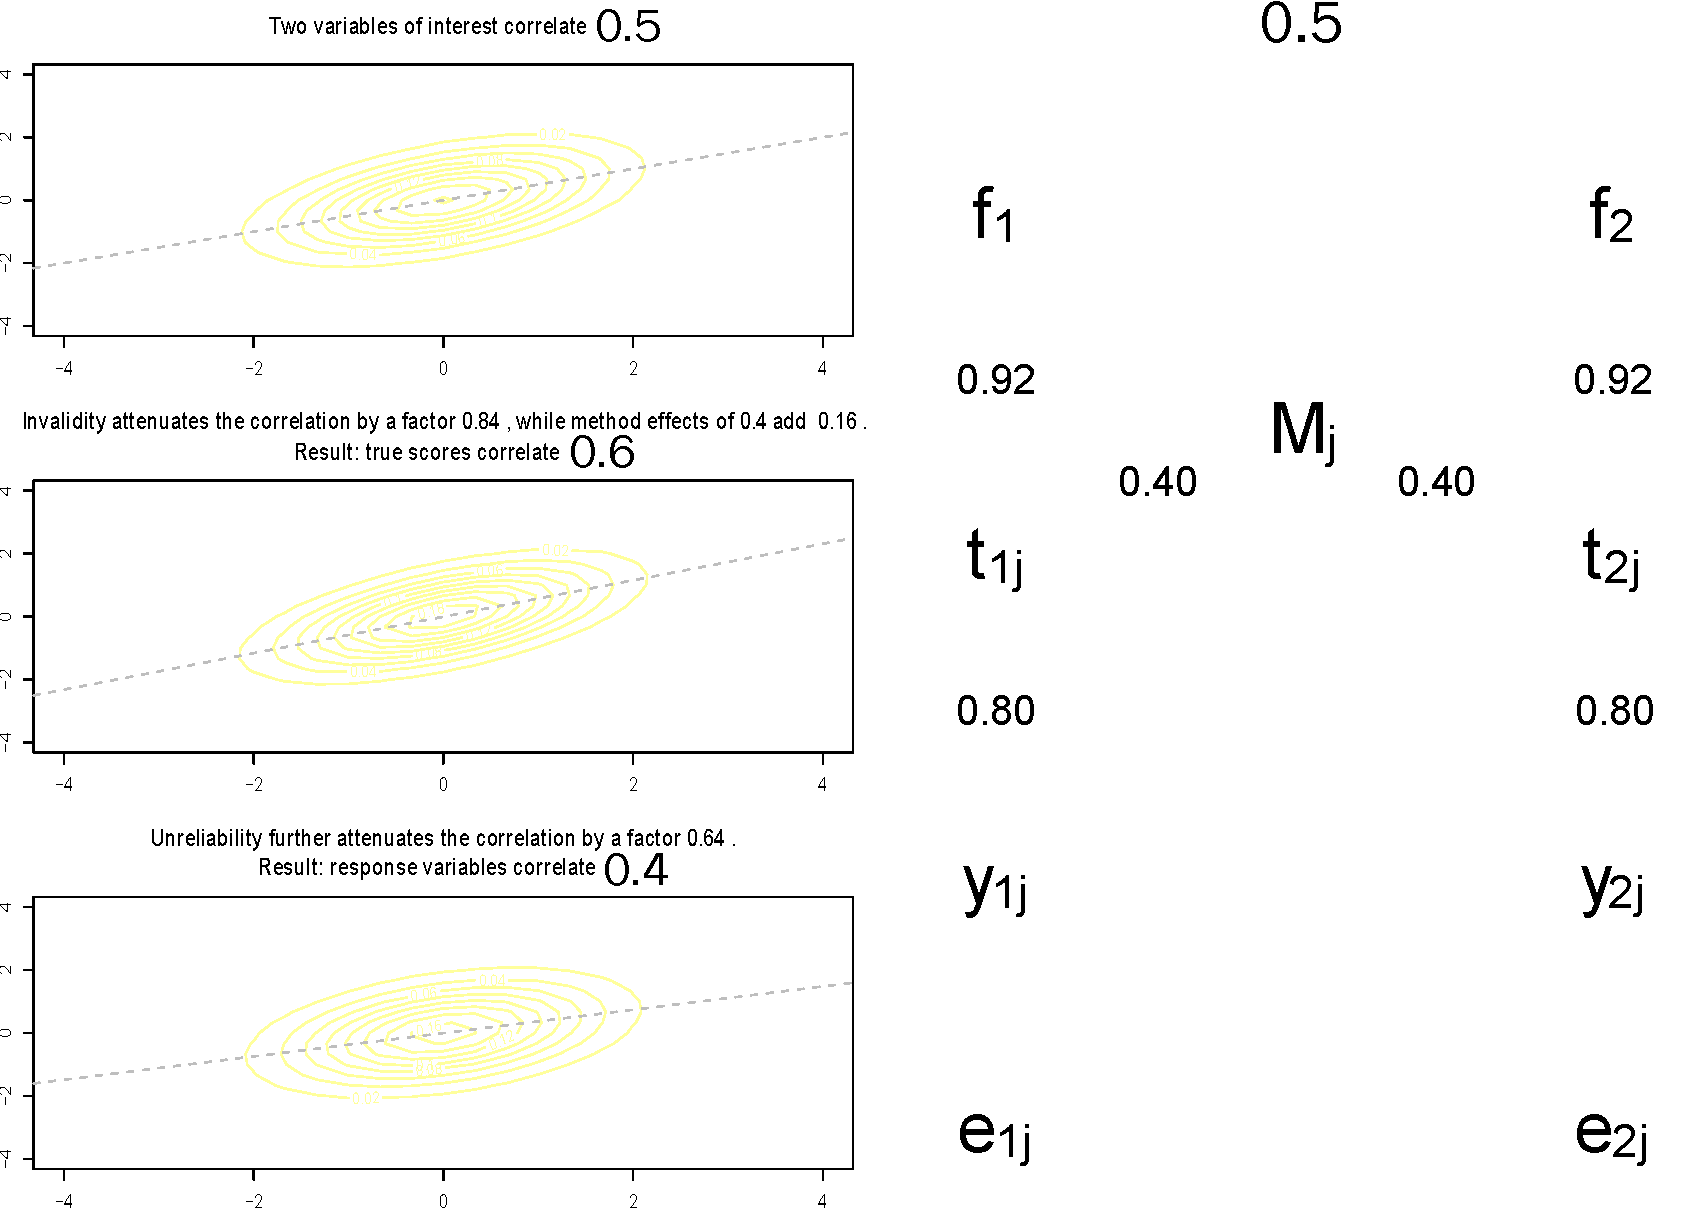
\includegraphics[height=8.3cm]{i/3_steps_together_CV.pdf}\\
\end{frame}

\subsection{Reliability, validity, and quality}
\begin{frame}	
	\frametitle{The basic response model}
	\begin{itemize}[<alert@+>]
		\item The quality coefficient $q$ is the product of the reliability and validity coefficients:
		\item $q = vr$
		\item The square $q^2$ is called the 'total quality' of a measure.
		\item It is the percentage of variance in the observed variable that can be explained by the latent variable of interest.
		\item The observed variables are assumed to be continuous.
	\end{itemize}
\end{frame}	

\subsection{Revised model for categorical data}
\begin{frame}
   \frametitle{The basic response model, revised}\pause
   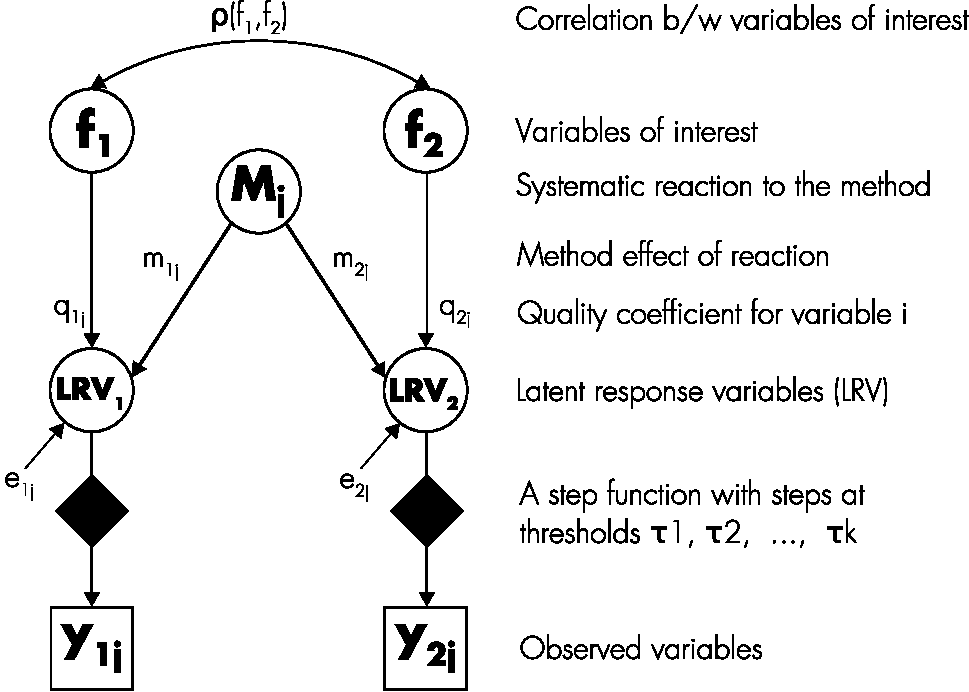
\includegraphics[height=7cm]{../latex/i/response_model_categorical.pdf}
\end{frame}


\begin{frame}
	\frametitle{Categorisation of continuous variables}

    Our model assumes that there are \emph{unobserved} continuous latent response variables (LRV) that have been categorised into the \emph{observed} categorical variables.

 \begin{columns}<2->[T]
 	\begin{column}{4.5cm} \textbf{country A}

	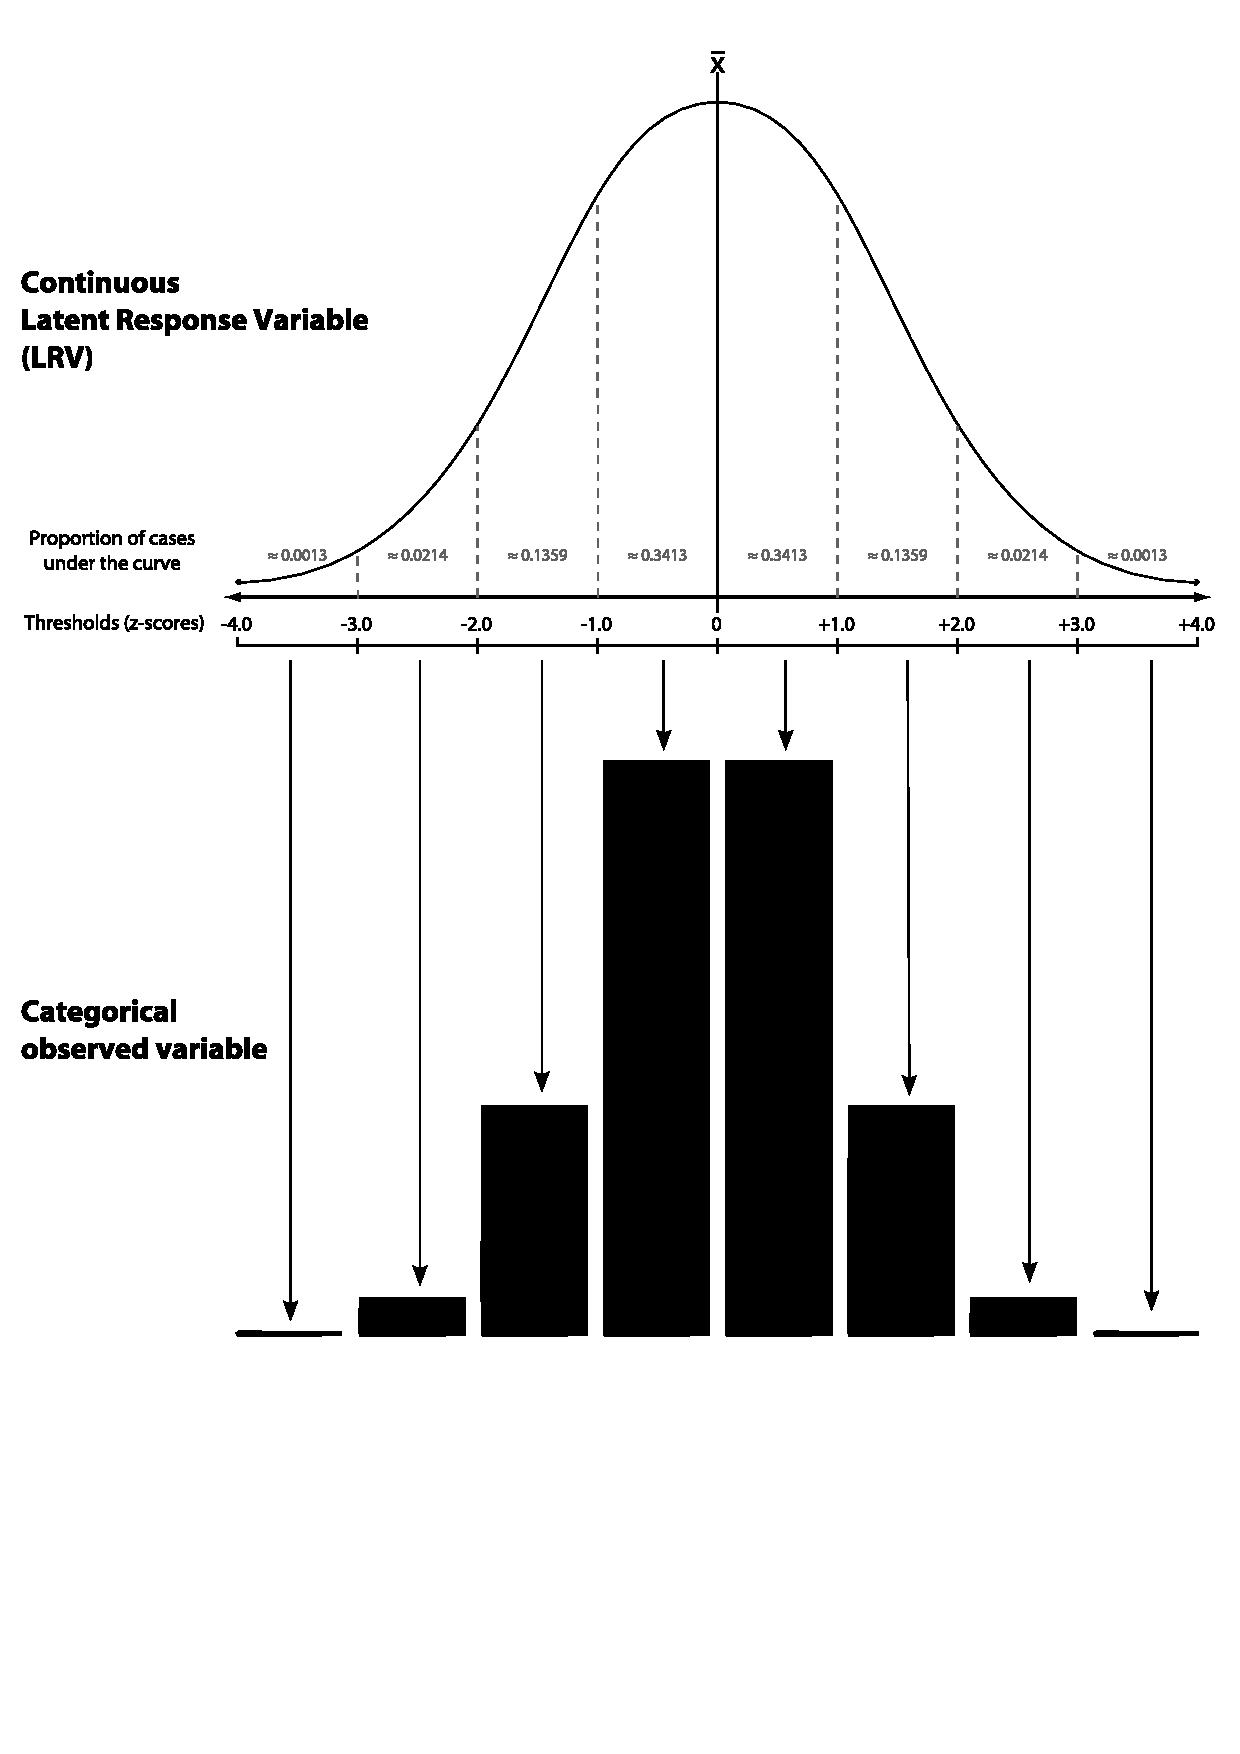
\includegraphics[width=4.5cm]{i/LRV-8cat.pdf}\end{column}
 	\begin{column}<3->{4.5cm} \textbf{country B}

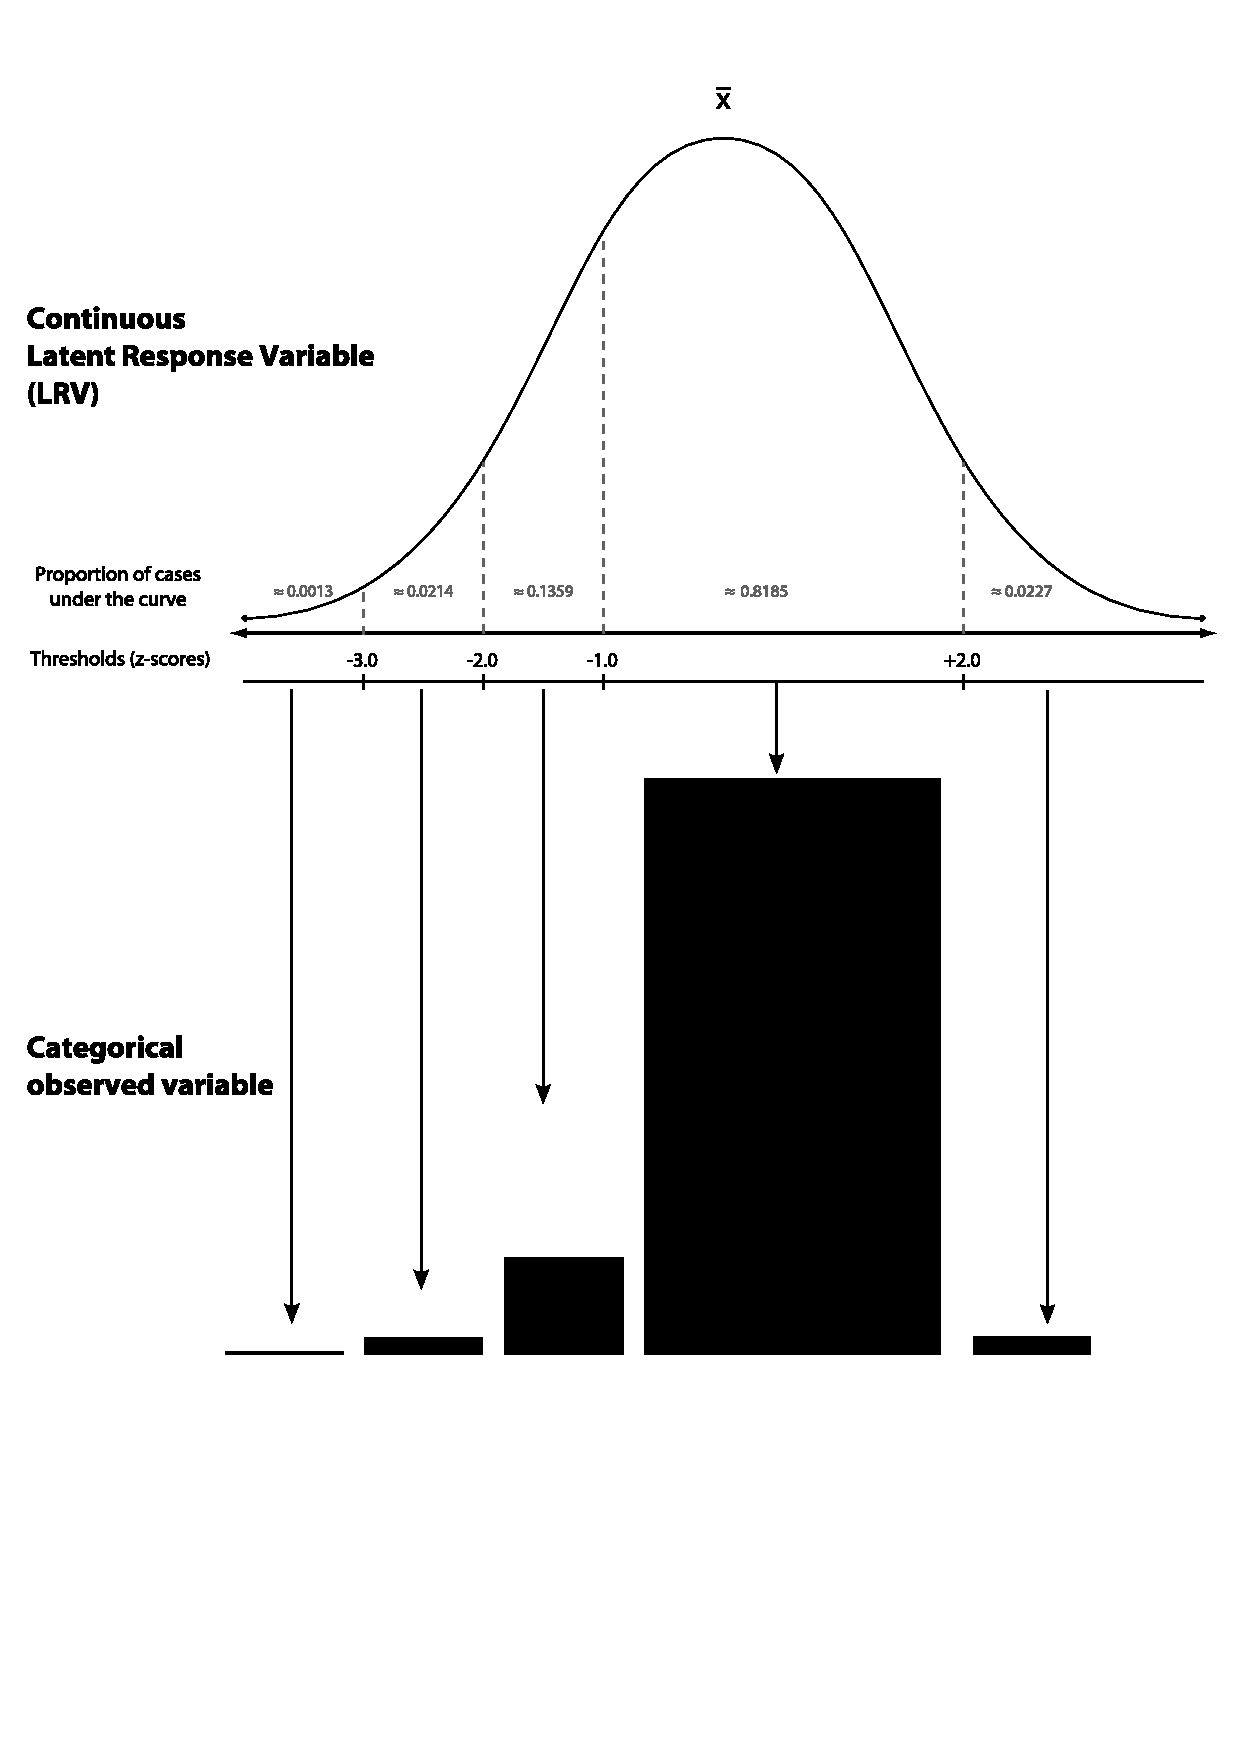
\includegraphics[width=4.5cm]{i/LRV-skew.pdf}
 	\end{column}
 \end{columns}
\end{frame}

\subsection{Revised model: Example}
\begin{frame}
   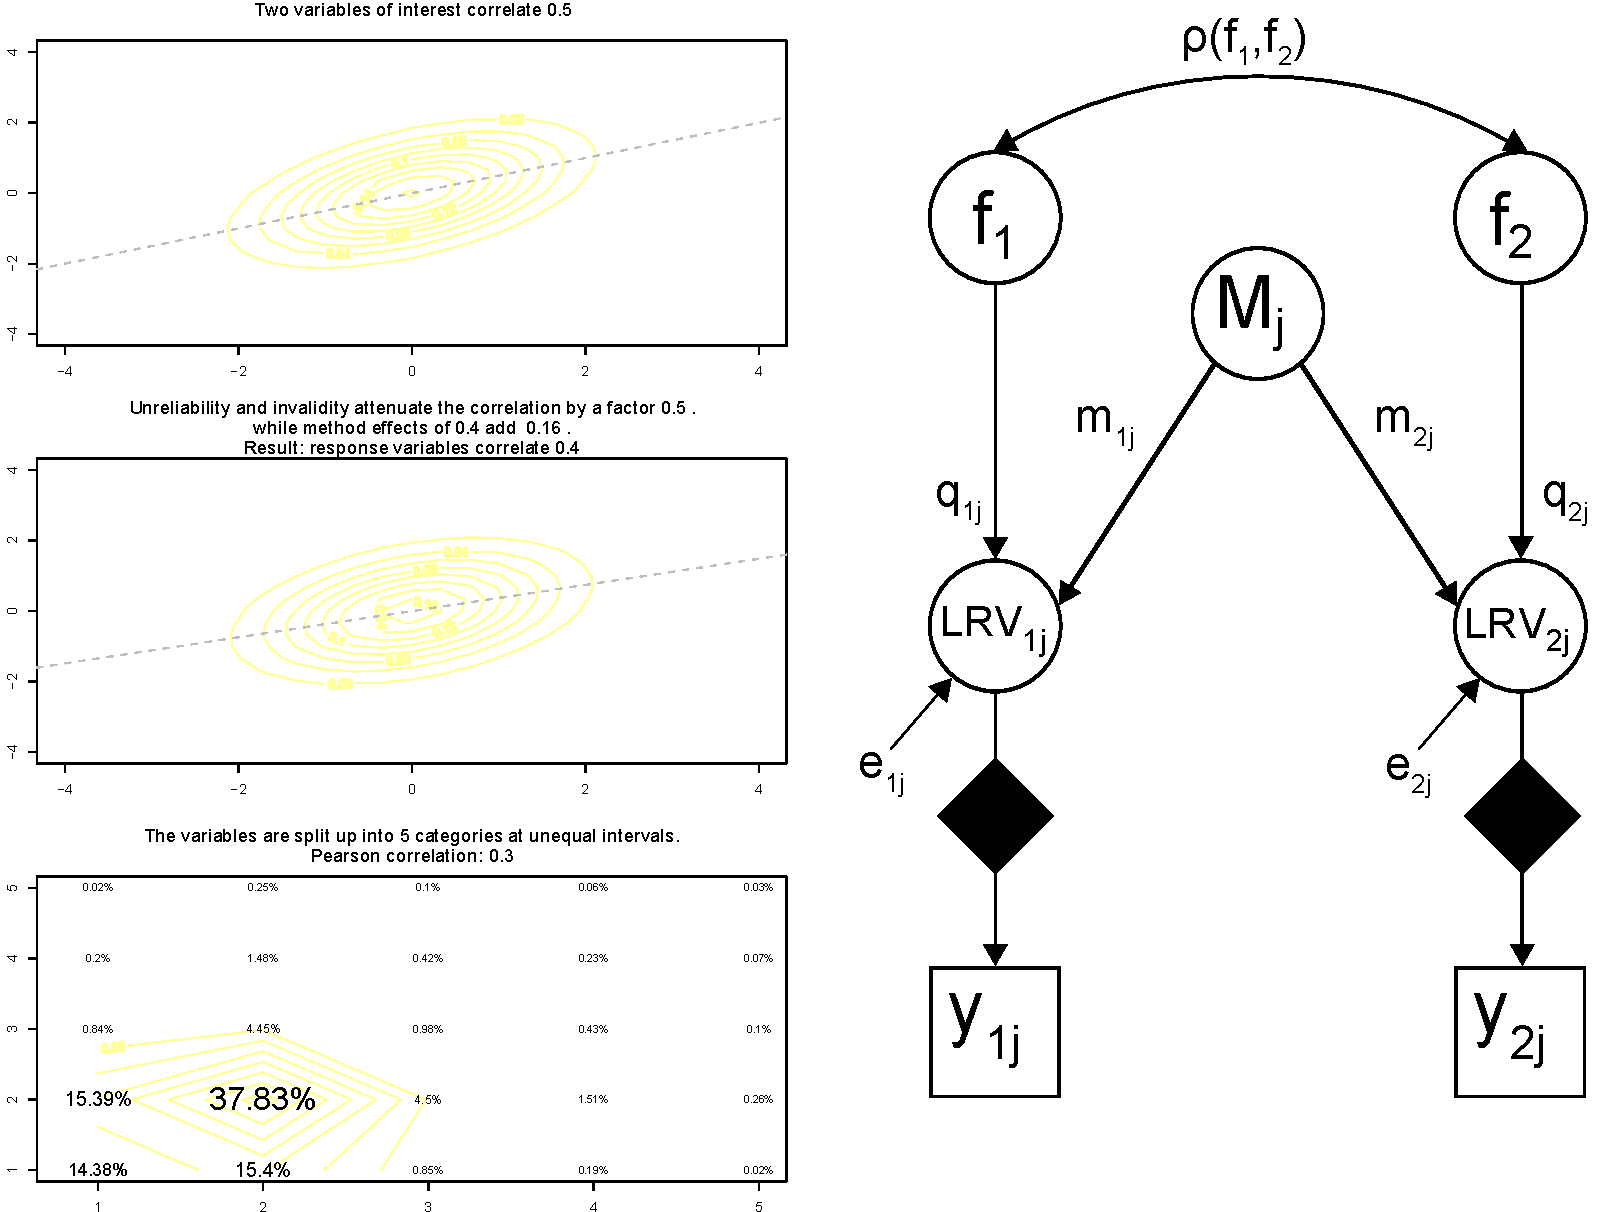
\includegraphics[height=8cm]{i/3_steps_together.pdf}
\end{frame}

\begin{frame}
\frametitle{Two countries with equal qualities but different means}
\begin{columns}<2->[T]
 	\begin{column}{5cm} 
	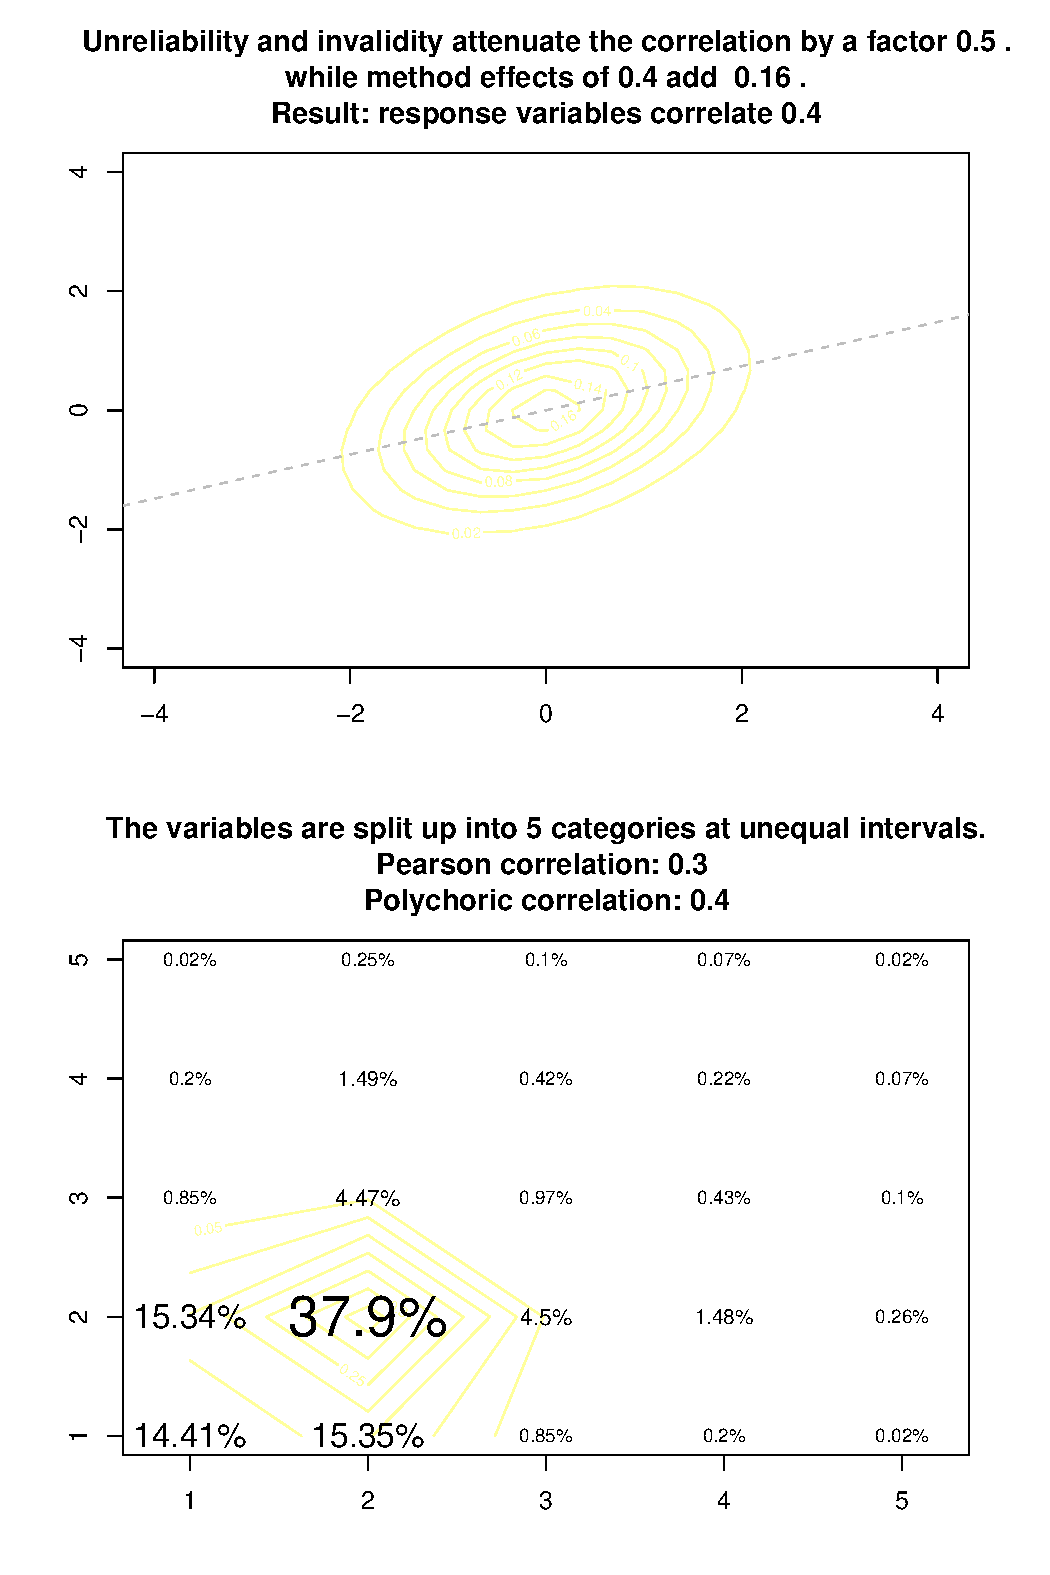
\includegraphics[width=5cm]{i/country_A.pdf}\end{column}
 	\begin{column}<3->{5cm} 
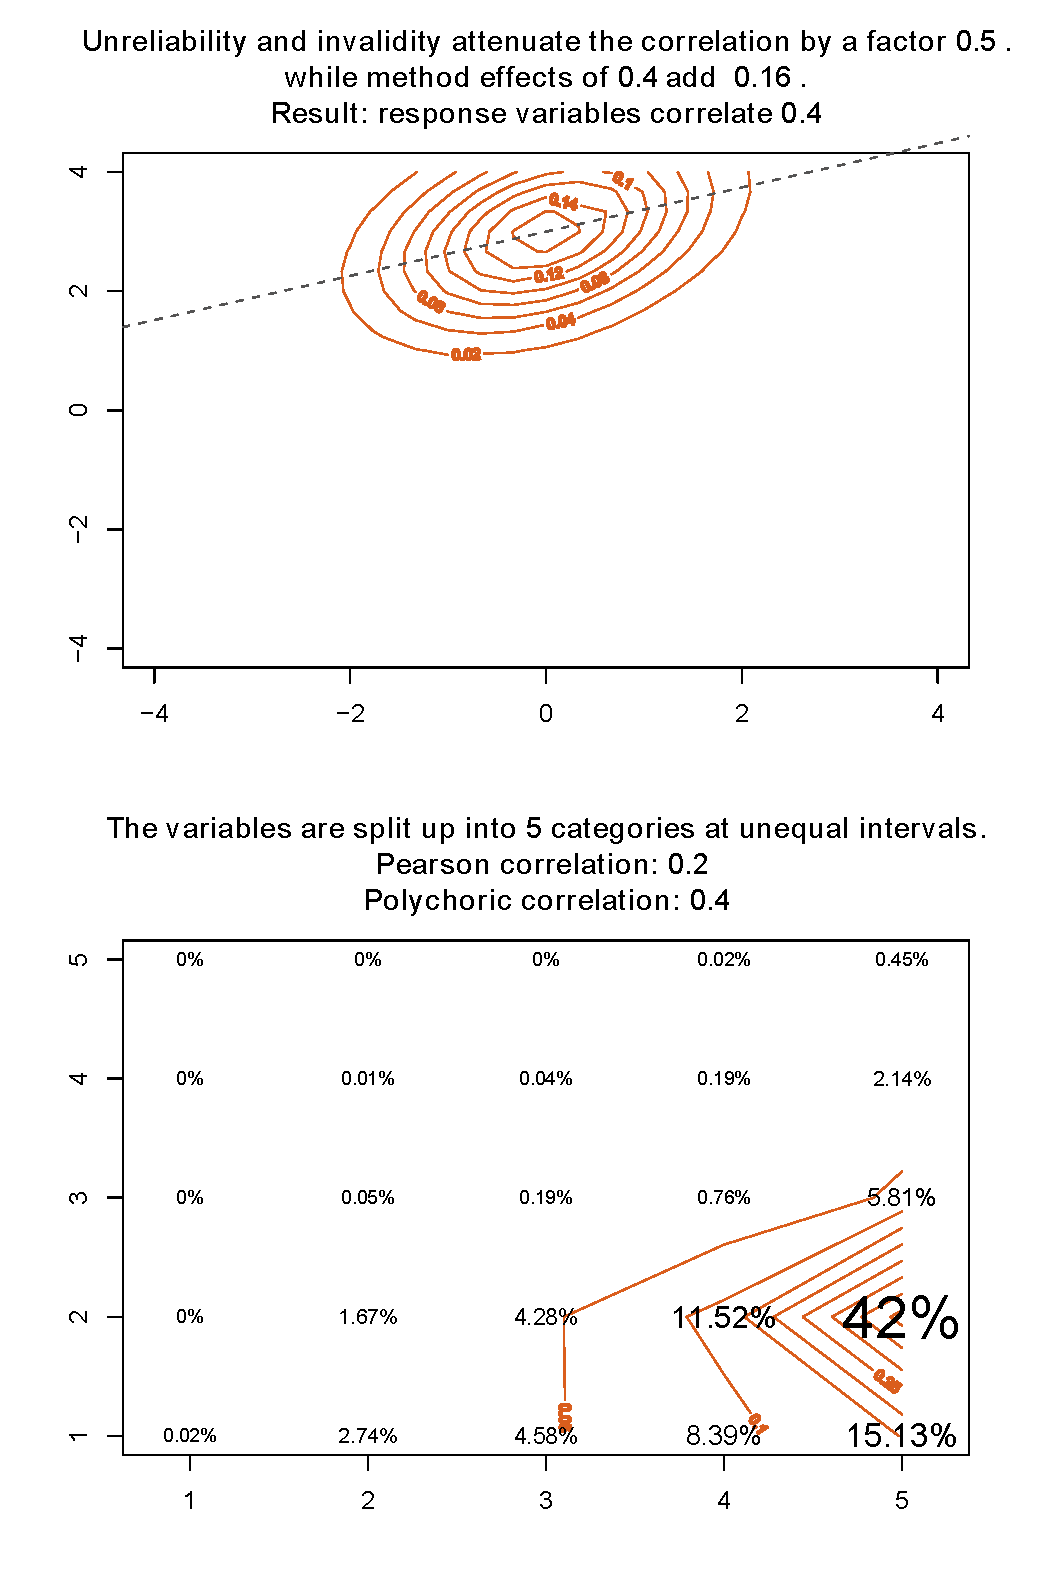
\includegraphics[width=5cm]{i/country_B.pdf}
 	\end{column}
 \end{columns}
\end{frame}

\subsection{Cross-cultural/time/group studies}
\begin{frame}	
	\frametitle{Categorical data in cross-country studies}
	\begin{itemize}[<alert@+>]
		\item The thresholds used earlier are taken from the estimates of a real experiment!
		\item If the thresholds are different, the observed means and (Pearson) correlations will differ also;
		\item Even a difference in \emph{means} across countries can cause an observed difference in Pearson correlations;
		\item If the assumption of normality holds true, the categorical response model (using polychoric correlations) corrects the LRV correlations;
		\item Whether this model is realistic is the topic of our other presentation...
	\end{itemize}
\end{frame}	

\section{Multitrait-multimethod experiments}
\begin{frame}

\textbf{\centering How can the quality and thresholds be estimated in different countries?}

\end{frame}

\subsection{An example experiment}
\begin{frame}
	\frametitle{First trait measured with three methods}
	\begin{tabular}{l}
		\hline
		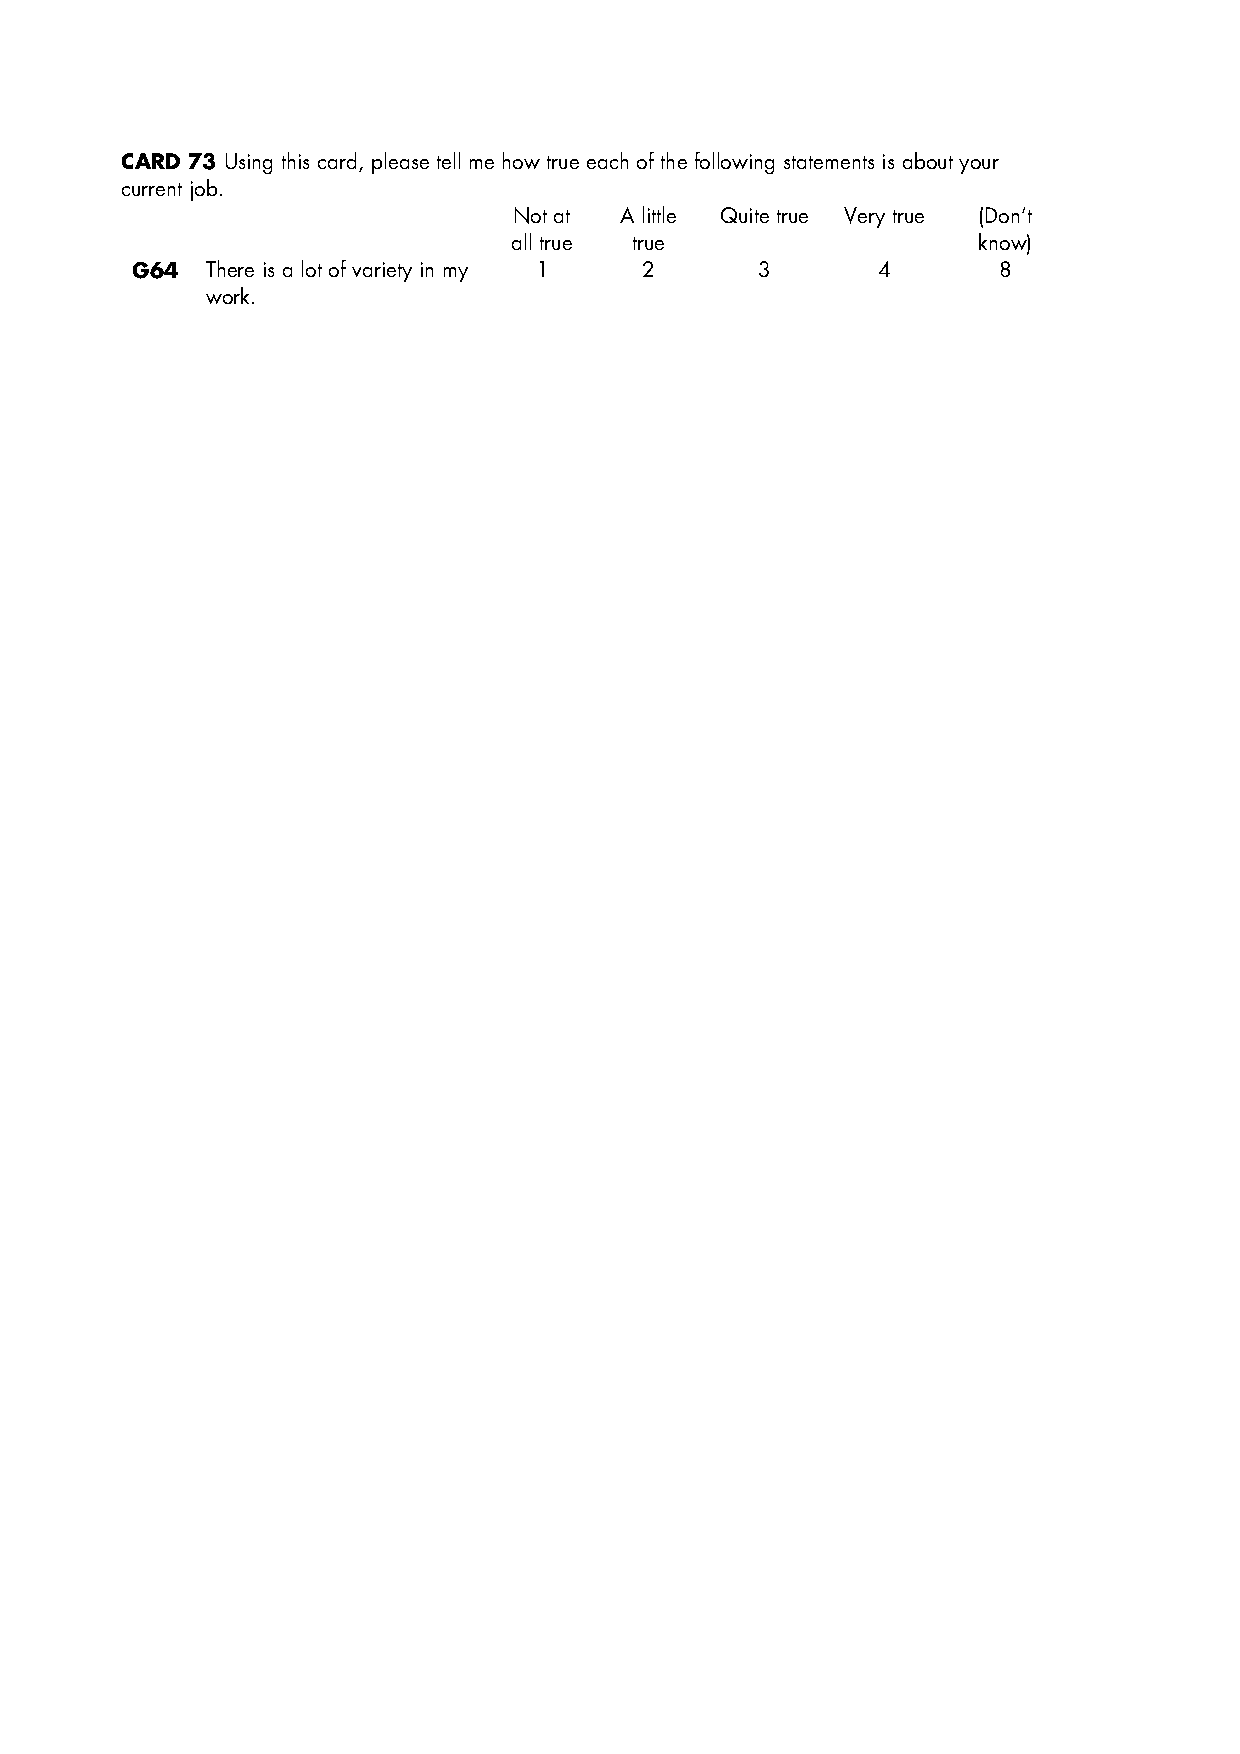
\includegraphics[width=8cm]{i/trait-1-m-1.pdf} \\\hline
		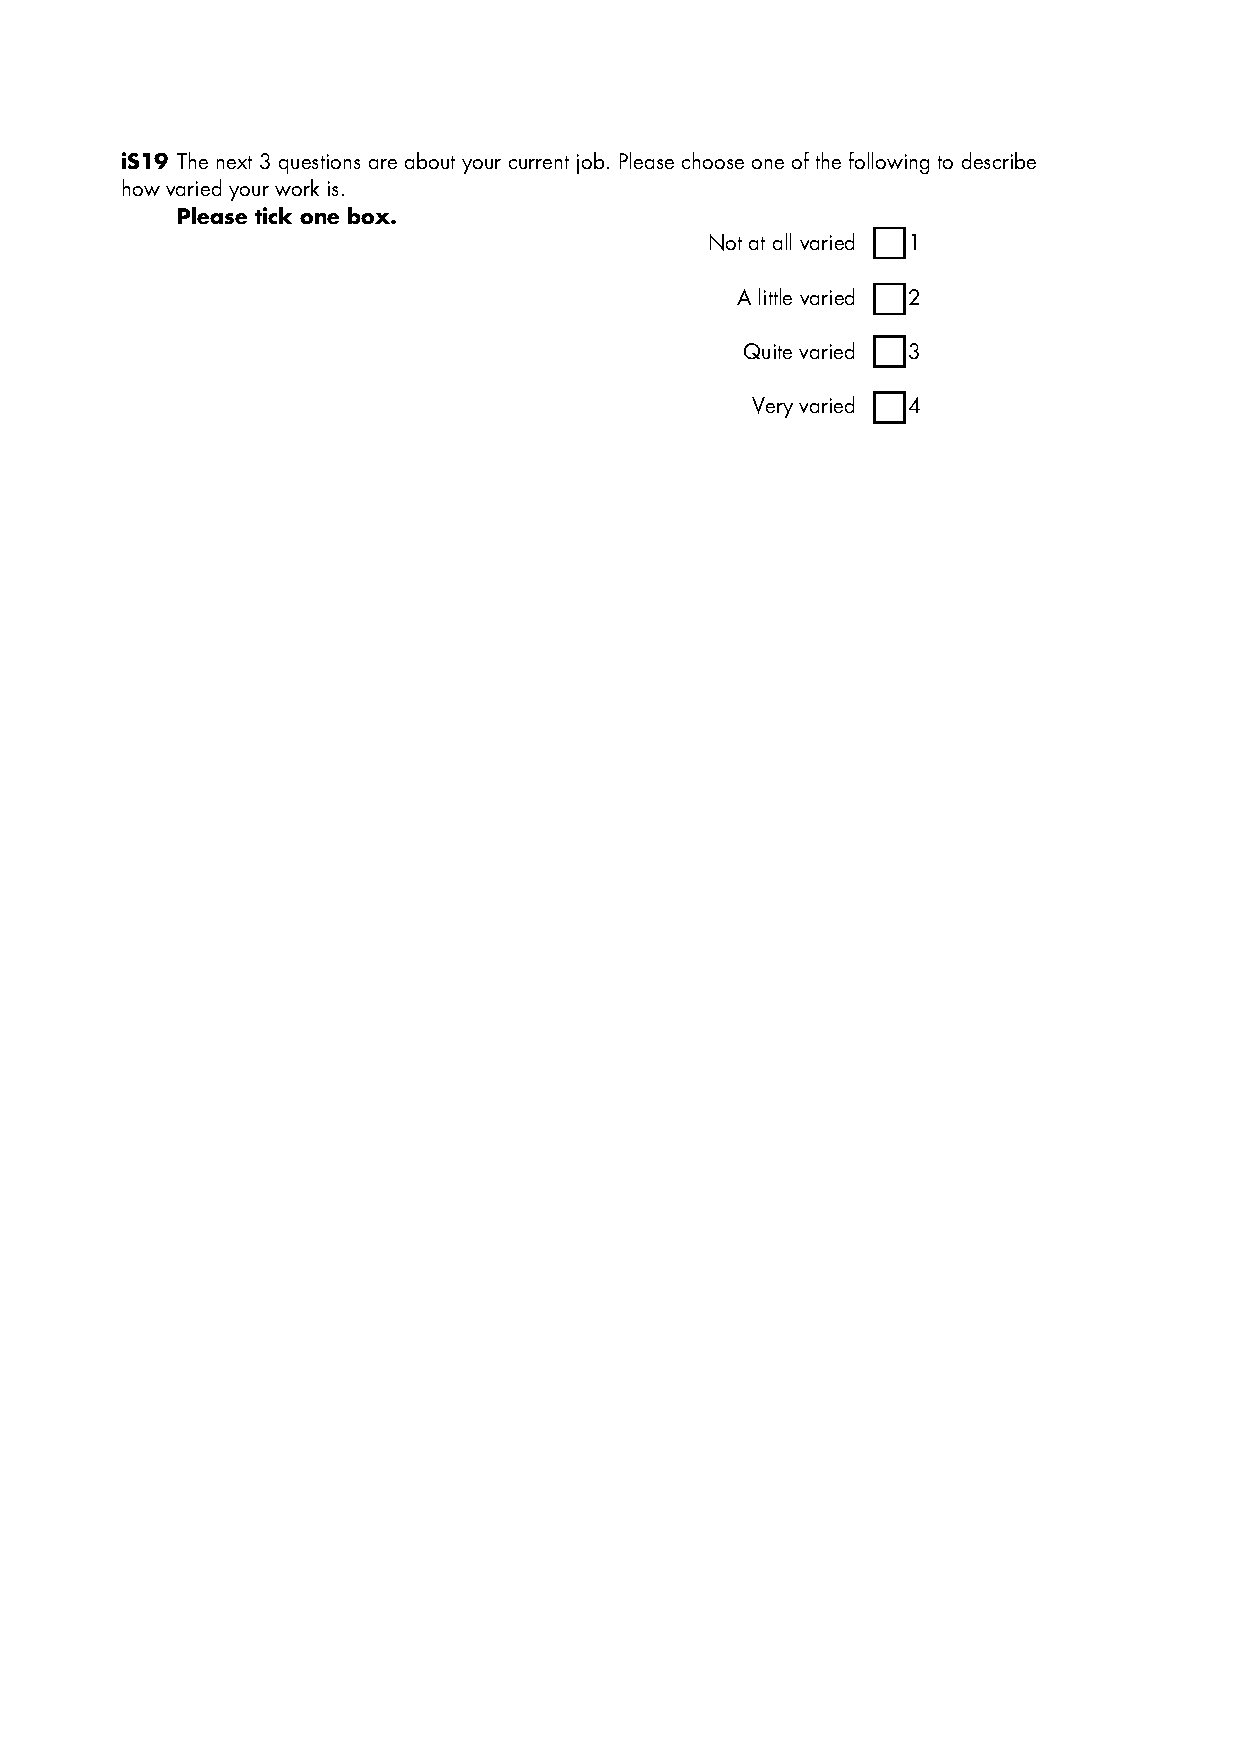
\includegraphics[width=8cm]{i/trait-1-m-2.pdf} \\\hline
		 
\includegraphics[width=8cm]{i/trait-1-m-3.pdf}\\
		\hline
	\end{tabular}
\end{frame}

\begin{frame}
	\frametitle{Three traits measured with first method}
		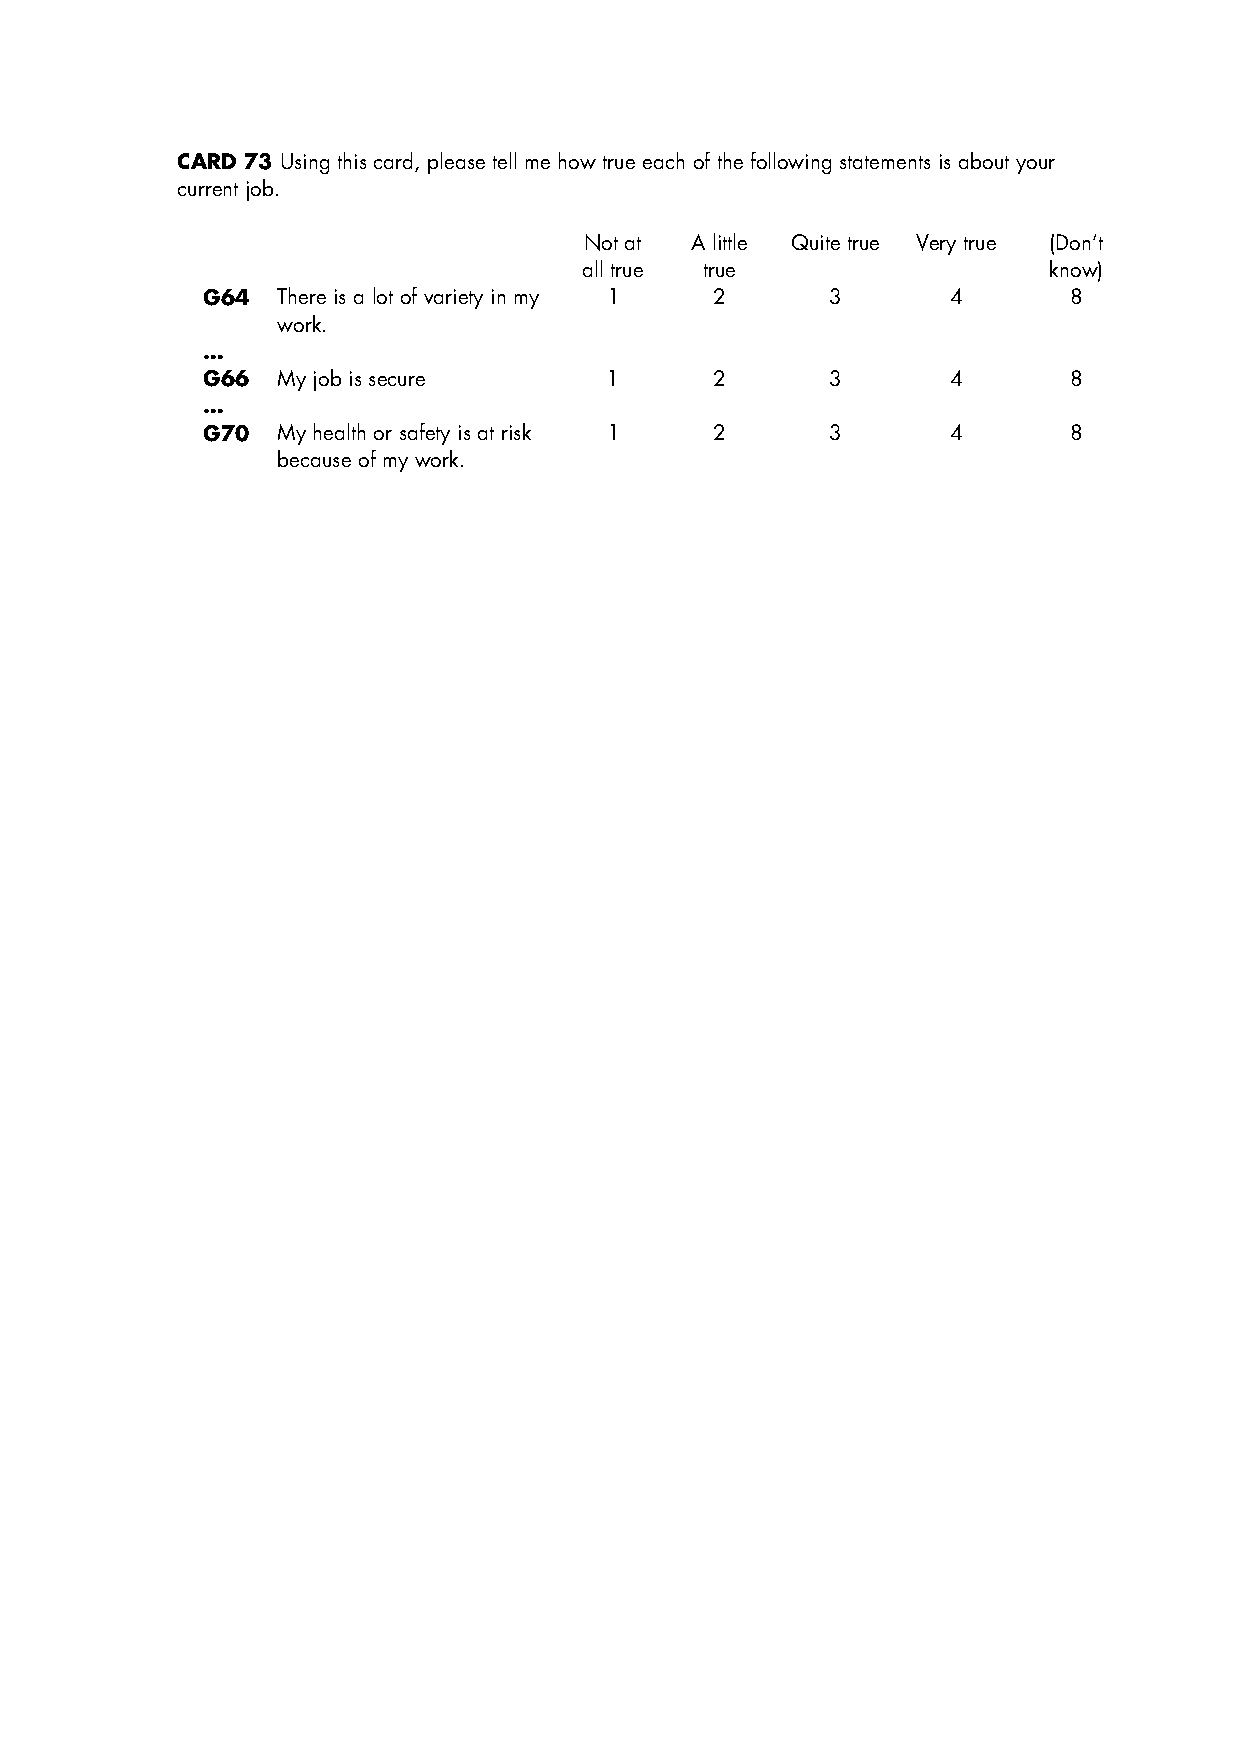
\includegraphics[width=11.2cm]{i/method-1.pdf}
\end{frame}

\begin{frame}
	\frametitle{Three traits measured with second method}
		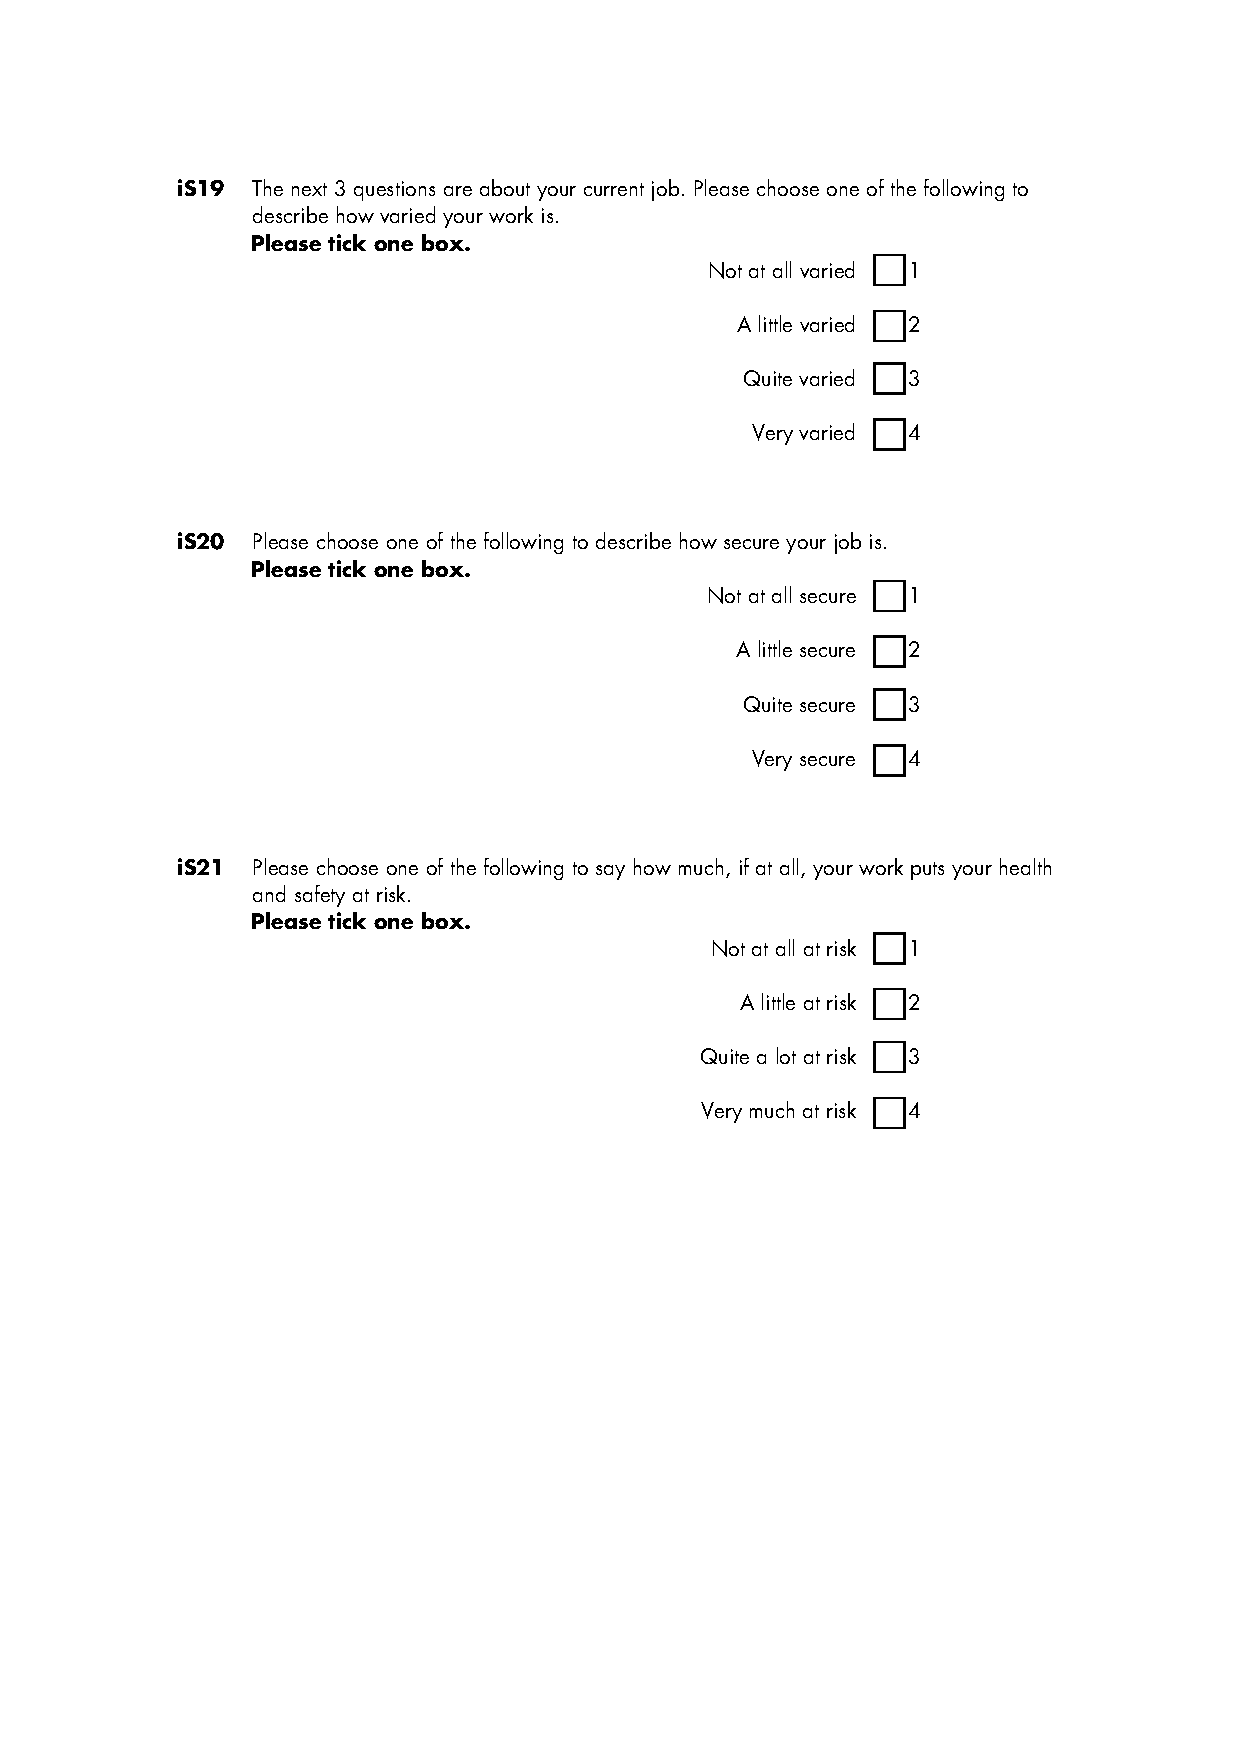
\includegraphics[height=7cm]{i/method-2.pdf}
\end{frame}

\begin{frame}
	\frametitle{Three traits measured with third method}
	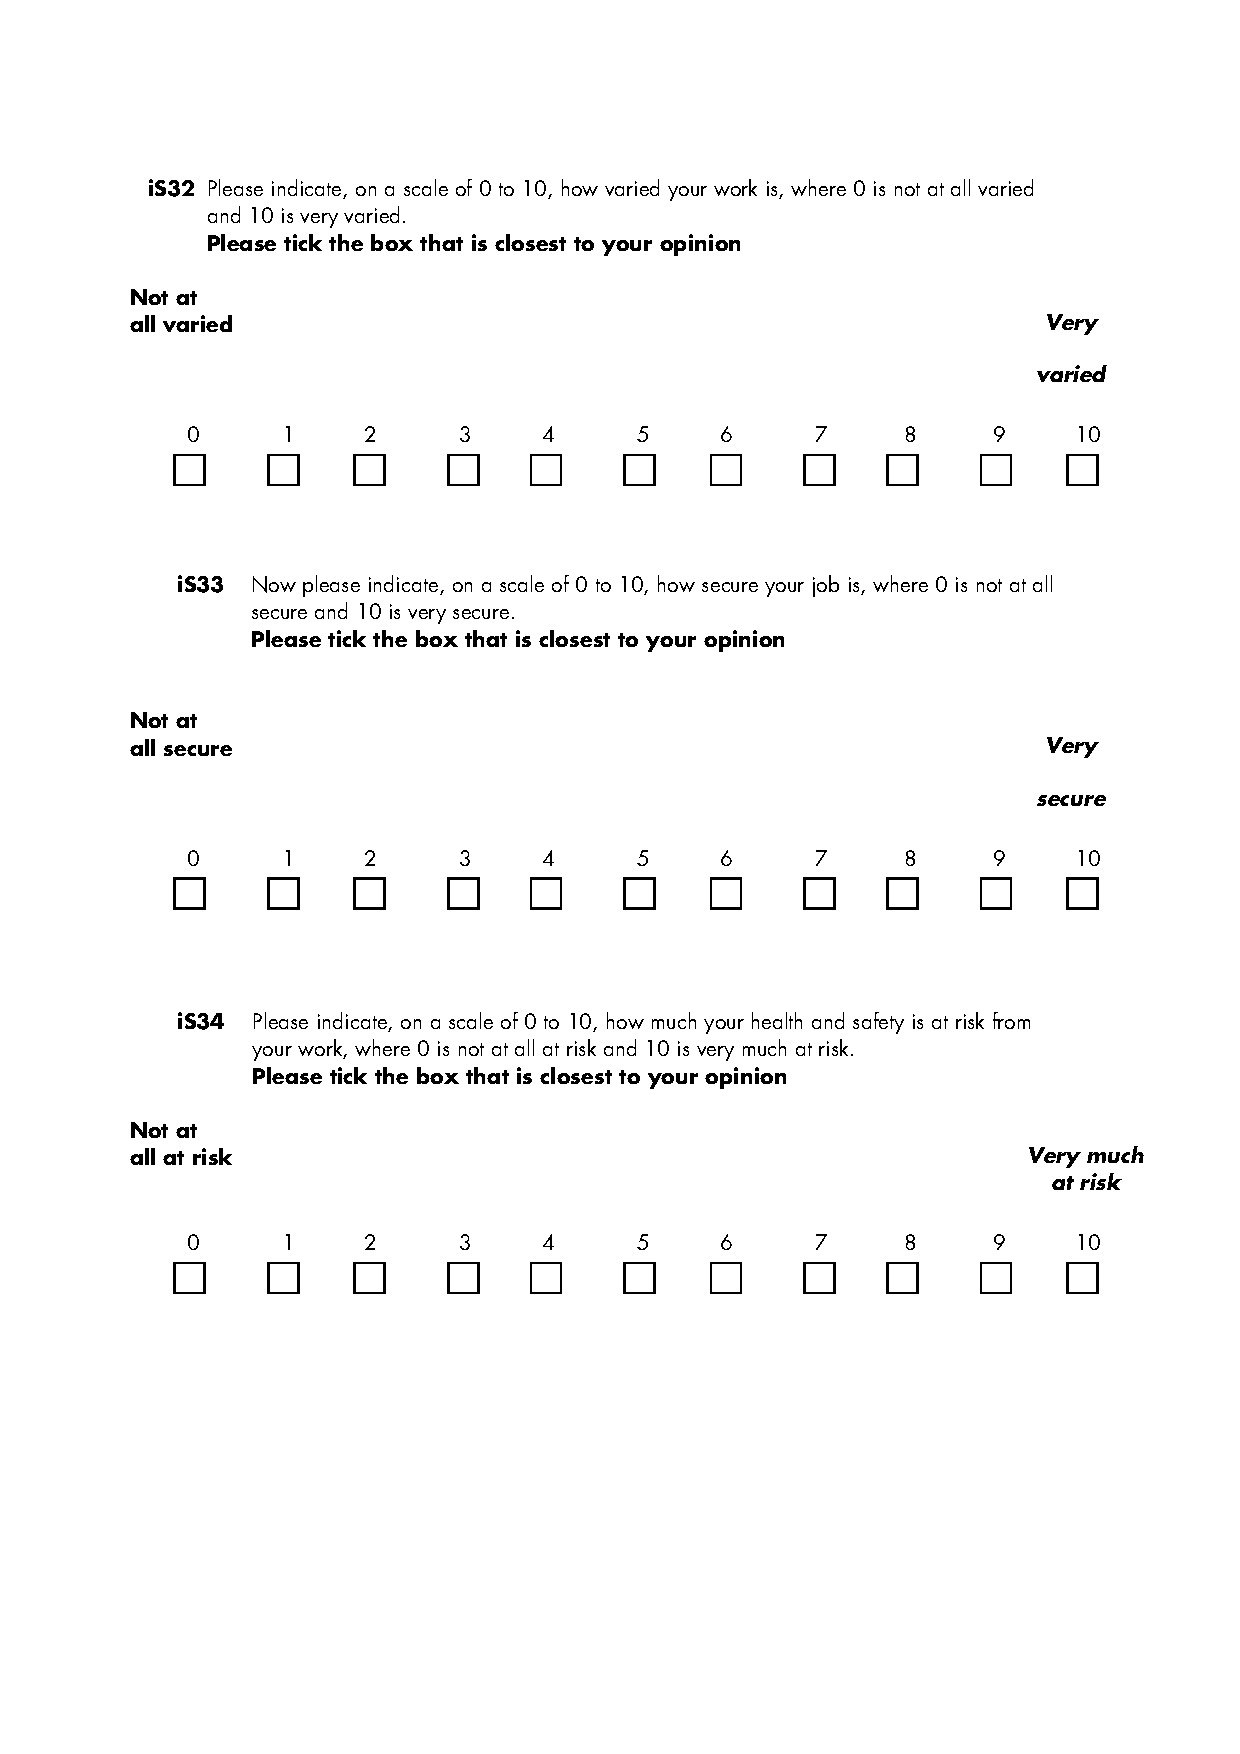
\includegraphics[height=7cm]{i/method-3.pdf}
\end{frame}


\subsection{Models}

\begin{frame}	
	\frametitle{\hypertarget{model}{Classic MTMM model}}
	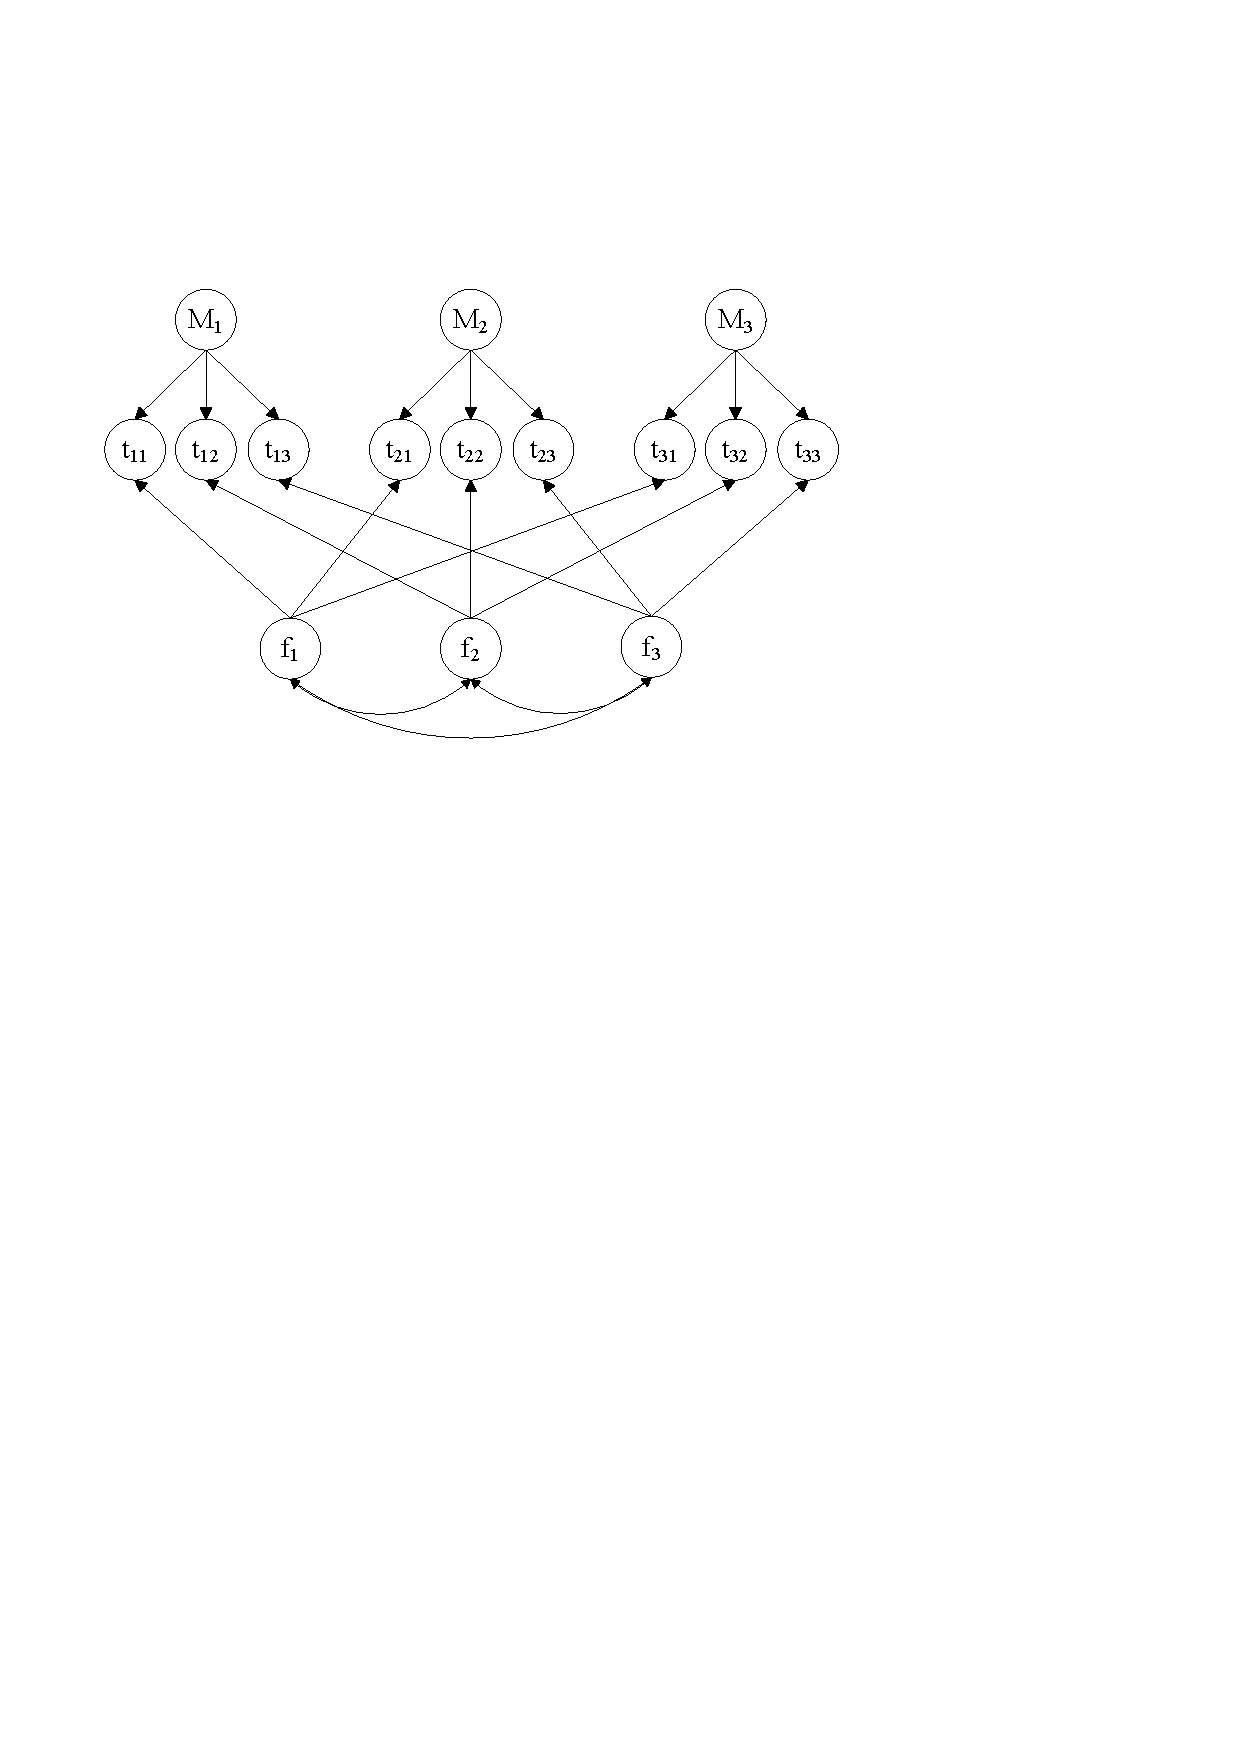
\includegraphics[height=7cm]{../latex/MTMM.pdf}
	\framezoom<1><2>(0cm,1.85cm)(.5cm,4.5cm)
	\framezoom<1><3>(0cm,0cm)(1cm,3cm)
\end{frame}	

\begin{frame}	
	\frametitle{MTMM model assumptions}
	\begin{itemize}[<alert@+>]
		\item No correlations among methods
		\item No correlations between traits and methods
		\item Equal method effects
		\item Linear and additive effects
		\item Normal errors, independent of all unobserved variables
%		\item All variables are continuous
	\end{itemize}
\end{frame}

\subsection{Results of the analyses across countries of the ESS round 2}
\begin{frame}
	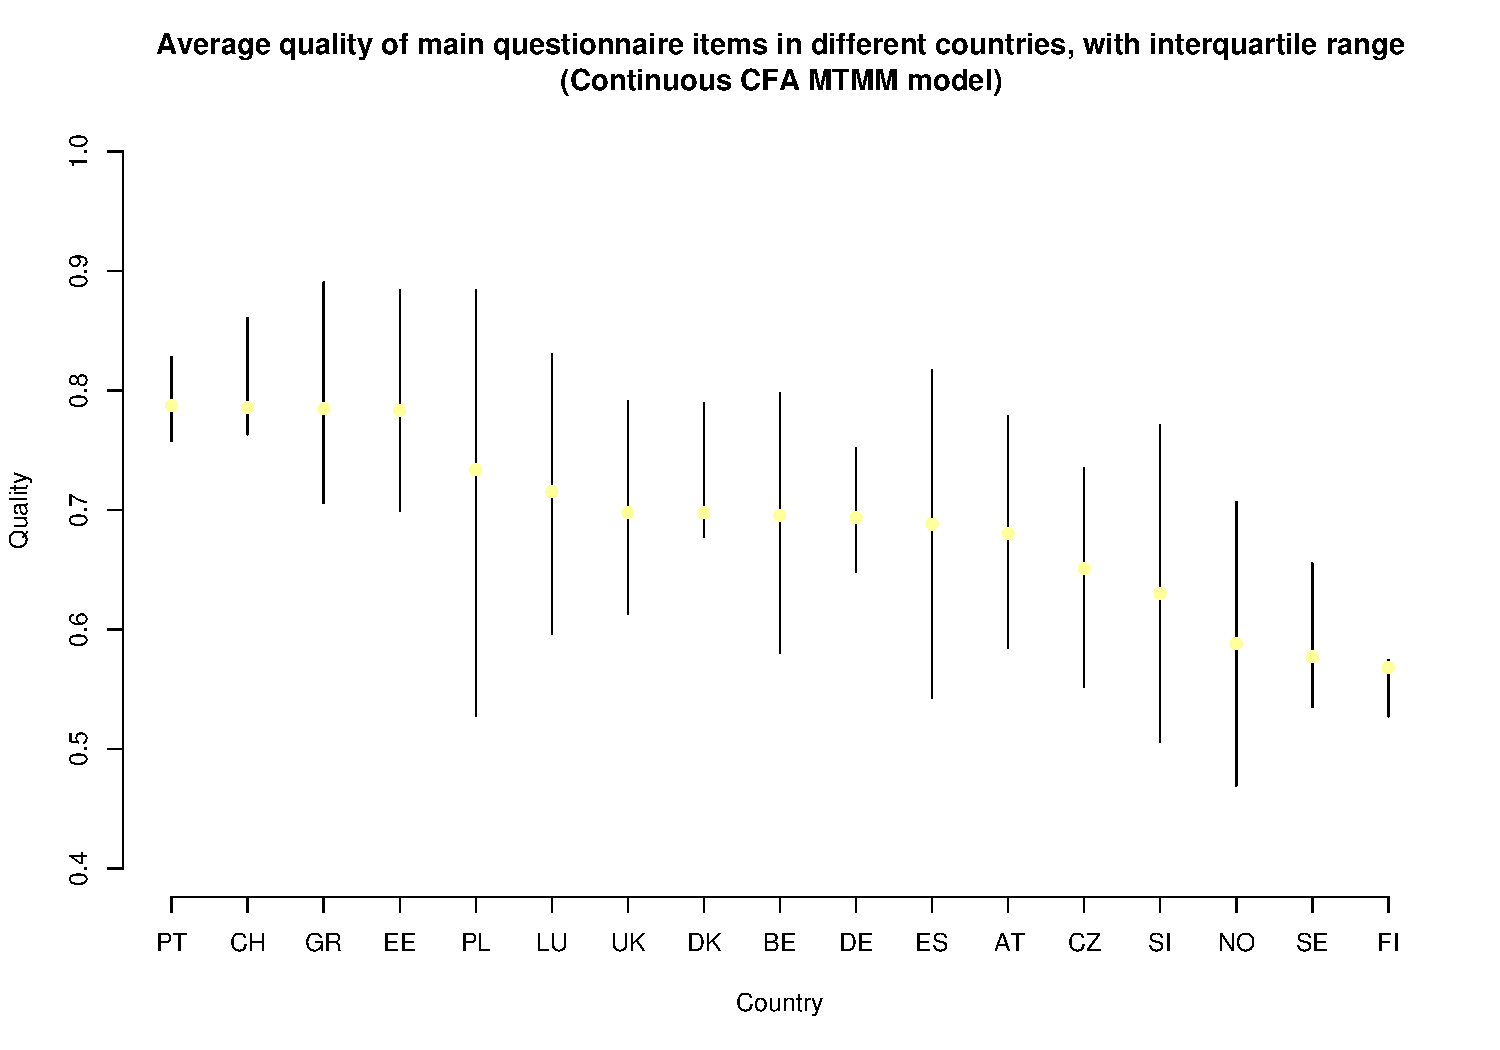
\includegraphics[height=8cm]{i/quality_plot.pdf}
\end{frame}


\begin{frame}	
\frametitle{Conclusions from the analysis of the \textbf{continuous} MTMM model}

	\begin{itemize}[<alert@+>]
		\item It is clear that categorization error may cause differences in Pearson correlations across countries;
		\item This can be expected to have its effect on the estimates of the MTMM model;
		\item Using the continuous model, quite some differences were indeed found in quality across countries;
		\item To what extent can these differences be explained by categorization errors?
		\item In order to quantify the differences between the models across countries we first define a measure called the `catgorisation factor':
	\end{itemize}
\end{frame}	

\subsection{Consequences of categorisation}
\begin{frame}
	\frametitle{The `categorisation factor'}
	\begin{itemize}
\item The quality was defined as:
		\item \begin{equation*}
q^2 = \frac{Var(f)}{Var(y)}.\label{eqn:relratio}
\end{equation*}
\item However, we have seen that $y$ is itself a categorization of an unobserved continuous variable ($LRV$), and therefore the above equation can be `decomposed' into
\item \begin{equation*}
q^2 =  \frac{ Var(f)}{Var(LRV)} \cdot \frac{Var(LRV)}{Var(y)}.		
\end{equation*}
	\item We call this ratio of the quality coefficient $q = v.r$ from the categorical model to the same coefficient from the continuous model the `categorisation factor'.
	\end{itemize}
\end{frame}

\begin{frame}
	\frametitle{The `categorisation factor'}

	\begin{equation}
	q^2 =  \frac{ Var(f)}{Var(LRV)} \cdot \frac{Var(LRV)}{Var(y)}.		
	\end{equation}

	\begin{itemize}
		\item It can be seen that the quality normally estimated from the continuous model is a product of two terms:
		\item $$
			q^2_{cont} = q^2_{categ} \cdot c,
		$$
		where $c$ is a categorisation factor.
\item If $c < 1$, the quality in the categorical model is higher than in the continuous model
		\item If $c > 1$, the quality in the categorical model is lower than in the continuous model
	\end{itemize}
\end{frame}


\begin{frame}
\frametitle{Analysis of the experiments}

	\begin{itemize}[<alert@+>]
		\item We analysed the 4 experiments from the ESS that involved variables with 5 categories or less
		\item The topics: role of women, doctors, political efficacy, job.

			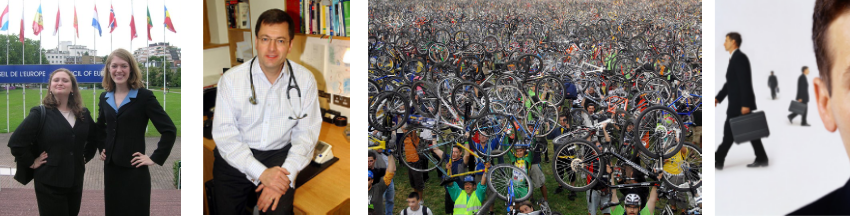
\includegraphics[width=10cm]{i/topics.png} 

	\item Compare the country with the highest quality to the country with the lowest quality for that experiment (not discussed here)
	\end{itemize}
\end{frame}


\subsection{Categorisation errors in the efficacy experiment}

\begin{frame}
\frametitle{Example: Quality ($q^2$)and method effects ($m$) in the efficacy experiment in Denmark}

Results of continuous MTMM model, main questionnaire (first method)

\begin{footnotesize}\begin{tabular}{llrrr}
\hline
 &  &  &   `Efficacy' & \\
&  &   Complex & Active & Mind\\
	   \hline
 &  $q^2$&   0.77 & 0.83 & 0.79\\
 &  $m$&   0.00 & 0.00 & 0.00\\
\hline
\end{tabular}


$df=19, \chi^2=40.0, p = 0.003$.
\end{footnotesize}
\end{frame}


\begin{frame}
\frametitle{Example: Efficacy experiment in Denmark}
\begin{footnotesize}
Polychoric correlations
\begin{tabular}{llrrrrrr}
 \hline
 &&\multicolumn{3}{c}{Method 1} & \multicolumn{3}{c}{Method 2}\\
 &&\multicolumn{3}{c}{$\overbrace{\hspace{90pt}}$} & \multicolumn{3}{c}{$\overbrace{\hspace{90pt}}$}\\
Method 1	& Complex 	& 1.00 \\
			& Active 	& -0.44 & 1.00 \\
			& Mind 		& -0.51 & 0.47 & 1.00 \\
Method 2	& Complex 	& 0.66 & -0.45 & -0.51 & 1.00 \\
			& Active 	& -0.44 & 0.74 & 0.46 & -0.51 & 1.00  \\
			& Mind 		& -0.52 & 0.51 & 0.67 & -0.56 & 0.56 & 1.00\\
 \hline
 \end{tabular}

Pearson correlations

\begin{tabular}{llrrrrrr}
 \hline
 &&\multicolumn{3}{c}{Method 1} & \multicolumn{3}{c}{Method 2}\\

 &&\multicolumn{3}{c}{$\overbrace{\hspace{90pt}}$} & \multicolumn{3}{c}{$\overbrace{\hspace{90pt}}$}\\
Method 1	& Complex 	& 1.00\\
			& Active 	&-0.38 & 1.00\\
			& Mind 		&-0.46 & 0.41 & 1.00\\
Method 2	& Complex 	& 0.60 & -0.37 & -0.44 & 1.00\\
			& Active 	&-0.39 & 0.67 & 0.40 & -0.43 & 1.00\\
			& Mind 		&-0.46 & 0.43 & 0.62 & -0.49 & 0.48 & 1.00\\
 \hline
 \end{tabular} 

$n \approx 916$
\end{footnotesize}

\end{frame}



\begin{frame}
\frametitle{Example: \% Increase in the correlations after correction for categorisation}

Efficacy experiment: Denmark

\begin{tabular}{llrrrrrr}
\hline
 &&\multicolumn{3}{c}{Method 1} & \multicolumn{2}{c}{Method 2}  \\
&&\multicolumn{3}{c}{$\overbrace{\hspace{90pt}}$} & \multicolumn{3}{c}{$\overbrace{\hspace{60pt}}$}\\
Method 1	& Complex 	& \\
			& Active 	& \textbf{16}\%\\
			& Mind 		& \textbf{11}\% & \textbf{15}\%\\
Method 2	& Complex 	& 10\% & 22\% & 16\%\\
			& Active 	& 13\% & 10\% & 15\% & \textbf{19}\%\\
			& Mind 		& 13\% & 19\% & 8\% &  \textbf{14}\% & \textbf{17}\%\\
\hline
\end{tabular}

Mean percentage increase of the polychoric correlations:  14.5\%

%> approx.power(2.187, 79.889, alpha=.05)
%[1] 0.05
\end{frame}


\begin{frame}
\frametitle{Example: Quality ($q^2$)and method effects ($m$) according to the continuous and categorical models, with categorisation factors}

\begin{footnotesize}\begin{tabular}{llrrr}
\hline
 &  &  &   `Efficacy' & \\
	   &  &   Complex & Active & Mind\\
	   \hline
 \multicolumn{2}{l}{Continuous analysis}\\
 &  $q^2$&  0.77 & 0.83 & 0.79  \\
 &  $m$&  0.00 & 0.00 & 0.00\\
\multicolumn{4}{l}{Categorical analysis} \\
 &  $q^2$&  0.63 & 0.70 & 0.63  \\
 &  $m$&  0.11 & 0.08 & 0.11 \\
\multicolumn{2}{l}{Categorisation factor}      &  & \\
 &  &  1.23 & 1.18 & 1.25 \\
\hline
\end{tabular}

\end{footnotesize}
\end{frame}


\begin{frame}
\frametitle{Correction for categorisation: conclusions}

\begin{itemize}[<alert@+>]
   \item The general `push'  is that all coefficients go up, because the polychoric correlations are in general higher than the Pearson correlations;
   \item But when method factors are taken into account, the coefficients can also go down;
   \item This happens especially when the method variance is very small (close to zero) in the continuous model, but larger in the categorical model;
	\item Would then expect countries with high quality in the continuous model to have a lower quality after correction for categorisation and vice versa.
	\end{itemize}
\end{frame}

\section{A meta-analysis of the categorisation error studies}
\begin{frame}\begin{center}
The categorisation factor, $q_{cat}/q_{cont}$ versus the quality:
 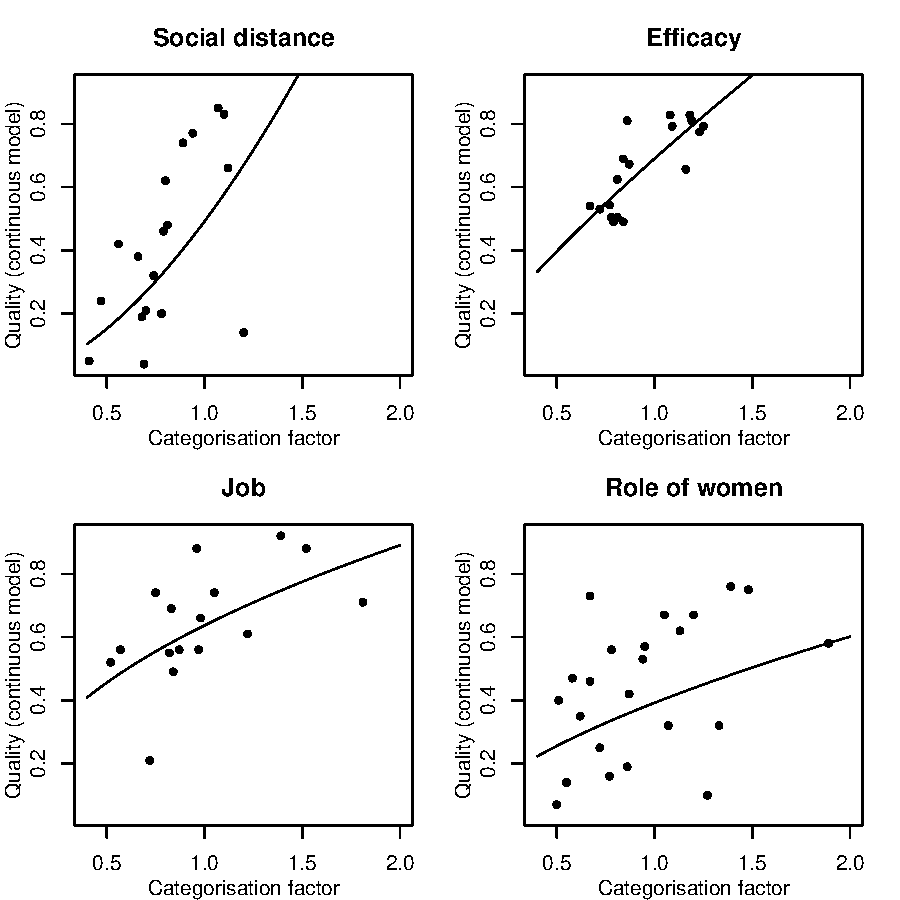
\includegraphics[height=7.4cm]{../latex/i/predict_q2.pdf} 
\end{center}
\end{frame}


\begin{frame}
\frametitle{Some implications of the findings}

\begin{itemize}[<alert@+>]
   \item Using discrete measures (with only a few categories) increased the apparent differences between countries using the continous factor model;
	\item Differences are smaller after correction for categorization;
	\item This means that either the continuous model gives misleading results regarding measurement invariance when analysing discrete data
	\item \textbf{OR}
	\item that the assumption of normality made in the `revised' (categorical) model is wrong.
\end{itemize}

\end{frame}


\begin{frame}
That's it for now. Moltes gr�cies per la seva atenci�!

\vspace{1em}\begin{footnotesize}
	\begin{columns}[T]
		\begin{column}{3cm}\centering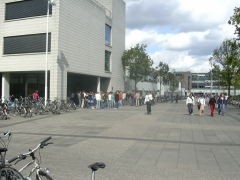
\includegraphics[width=2.55cm]{i/uvt_fac.jpg} 

Tilburg\end{column}
		\begin{column}{3cm}\centering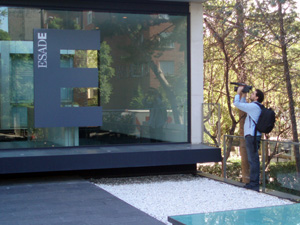
\includegraphics[width=2.5cm]{i/esade_fac.jpg} 

Barcelona\end{column}
	\end{columns}		
\end{footnotesize}
\end{frame}

\section{Epilogue}

\begin{frame}
\frametitle{The latent traits}

Estimated correlations between the latent traits under the two different models in the example given before

\begin{tabular}{lrrr}
\hline
	 & Complex & Active & Mind\\
\hline
Continuous model & 1\\
&-.63  &     1\\
&-.75   &    .66   &   1\\
&\\
Categorical model &1 \\
&-.63 & 1\\
&-.75  & .70 & 1\\
\hline
\end{tabular}
\end{frame}

\section{Conclusion}

\begin{frame}

\frametitle{Conclusions}
\begin{itemize}[<alert@+>]
   \item It was possible to split the measurement error model into three parts:
      \begin{itemize}
	 \item A part due to random errors;
	 \item A part due to systematic errors;
	 \item A part due to splitting the variable into just a few categories.
      \end{itemize}
   \item The estimates one gets can differ, and not always in the way one might expect;
   \item The correlations between the latent traits corrected for measurement error \textbf{in this experiment} were robust to the model specification;
   \item This suggests either model will provide a correct (or at least similar) inference about the variables of interest in this particular case;
	\item One cannot expect this to be the case in general, however.
\end{itemize}
\end{frame}


\begin{frame}
\frametitle{Further study, problems}
	\begin{itemize}[<alert@+>]
				\item Investigate normality assumption (tests indicate possible issues), linearity;
				\item Unobserved heterogeneity;
				\item Prediction of the data quality based on characteristics of the question.
			\end{itemize}
\end{frame}

\begin{frame}
 \frametitle{The final goal: Survey Quality Predictor (SQP)}

	\begin{enumerate}[<alert@+>]
		\item Estimate the model for all experiments
		\item Save the reliability, validity, and method effect coefficients
		\item Relate the coefficients to different aspects of the question
			\begin{itemize}[<4-|alert@+>]
				\item Complexity of the sentence: no. words/sentence, avg. no. syllables, ...
				\item Response scale: type, no. categories, ...
				\item Formulation of the request: agree-disagree, extra information, ...
				\item Data collection method: computer assisted, interviewer present, ...
			\end{itemize}
		\item Predict the quality of survey questions from their characteristics (SQP)
		\item Improve survey questions
		\item \texttt{http://www.sqp.nl} 
	\end{enumerate}
\end{frame}


\begin{frame}
 \frametitle{References of interest}

\begin{thebibliography}{10}
\bibitem{Saris2008}
Saris, Willem, Albert Satorra, and William van der Veld
\newblock Testing Structural Equation models or Detection of misspecifications? 
\newblock Forthcoming in \emph{Structural Equation Modeling: an interdisciplinary journal}.
\end{thebibliography}

\end{frame}


\end{document}
